\documentclass[11pt,letterpaper]{book}
\setlength{\oddsidemargin}{0.5in}
\setlength{\topmargin}{0in}
\setlength{\evensidemargin}{0.3in}
\setlength{\textwidth}{5.75in}
\setlength{\textheight}{8.5in}
%\setlength{\oddsidemargin}{1.25in}
%\setlength{\evensidemargin}{0.5in}

% don't do this \usepackage{times}    % Better fonts than Computer Modern
\renewcommand{\sfdefault}{phv}
\renewcommand{\rmdefault}{ptm}
% don't replace tt -- old is better \renewcommand{\ttdefault}{pcr}
%\usepackage{apalike}
\usepackage{pslatex}
\usepackage{techref}
\usepackage{epsfig}
\usepackage{verbatim}
\usepackage{moreverb}
\usepackage{graphicx}
\usepackage{xspace}
\usepackage{multicol}
\usepackage{color}
\usepackage{html}
\usepackage{version}
\usepackage{makeidx}
%\usepackage{showidx}
\usepackage[chapter]{algorithm}
\floatname{algorithm}{Listing}

\usepackage{syntax}

\widowpenalty=1000
\clubpenalty=1000

\usepackage{fancyhdr}
\pagestyle{fancy}
\fancyhead[LE,RO]{\bfseries\thepage}
\fancyhead[LO]{\bfseries\rightmark}
\fancyhead[RE]{\bfseries\leftmark}
\fancyfoot[C]{\bfseries Open Shading Language Specification}
\renewcommand{\footrulewidth}{1pt}


\def\langname{Open Shading Language\xspace}
\def\product{{\sffamily Open Shading Language}\xspace}
\def\versionnumber{0.9}
\def\productver{\product\ {\sffamily \versionnumber}\xspace}


\title{ 
{\Huge{\bf \product}
%\textregistered\ 
{\bf\sffamily \versionnumber} \medskip \\ \huge 
Language Specification
%\\ \large (CONFIDENTIAL --- draft in progress) 
} \bigskip }
\author{
\copyright\ Copyright 2009 Sony Pictures Imageworks Inc., et al. All rights reserved.
 \bigskip \\
\vspace{1in} \\
Editor: Larry Gritz \\
\emph{lg@imageworks.com}
 \bigskip \\
}
\date{{\large Date: 11 January, 2010 \\
(with corrections, 8 February, 2010)
}}


%%%%%%%%%%%%%%%%%%%%%%%%%%%%%%%%%%%%%%%%%%%%%%%%%%%%%%%%%%%%%%%%%%%%%%%%%%
% Larry's favorite LaTeX macros for making technical books.  These have
% been refined for years, starting with SIGGRAPH course notes in the
% '90's, further refined for _Advanced RenderMan_.
%
% Please use or modify this at will.
%%%%%%%%%%%%%%%%%%%%%%%%%%%%%%%%%%%%%%%%%%%%%%%%%%%%%%%%%%%%%%%%%%%%%%%%%%

%
% Define typesetting commands for filenames and code
%
% Just like Advanced RenderMan -- all code in courier, keywords in text
%    courier but not bold.
\def\codefont{\ttfamily}	% font to use for code
\def\ce{\codefont\bfseries}	% emphasize something in code


%
% Define typesetting commands for filenames and code
%
\def\cf{\codefont}		% abbreviation for \codefont
\def\fn{\codefont}		% in-line filenames & unix commands
\def\kw{\codefont}      	% in-line keyword

\newcommand{\var}[1]{{\kw \emph{#1}}}  % variable
\newcommand{\qkw}[1]{{\kw "#1"}}       % quoted keyword



% Define some environments for easy typesetting of small amounts of
% code.  These are mostly just wrappers around verbatim, but the
% different varieties also change font sizes.
\newenvironment{code}{\small \verbatimtab}{\endverbatimtab}
\newenvironment{smallcode}{\small \renewcommand{\baselinestretch}{0.8} \verbatimtab}{\endverbatimtab \renewcommand{\baselinestretch}{1}}
\newenvironment{tinycode}{\footnotesize \renewcommand{\baselinestretch}{0.75} \verbatimtab}{\endverbatimtab \renewcommand{\baselinestretch}{1}}

\begin{htmlonly}
\renewenvironment{code}{\begin{verbatim}}{\end{verbatim}}
\newenvironment{smallcode}{\begin{verbatim}}{\end{verbatim}}
\newenvironment{tinycode}{\begin{verbatim}}{\end{verbatim}}
\end{htmlonly}

\newcommand{\includedcode}[1]{{\small \verbatimtabinput{#1}}}
\newcommand{\smallincludedcode}[1]{{\small \renewcommand{\baselinestretch}{0.8} \verbatimtabinput{#1} \renewcommand{\baselinestretch}{1}}}
\newcommand{\tinyincludedcode}[1]{{\footnotesize \renewcommand{\baselinestretch}{0.75} \verbatimtabinput{#1} \renewcommand{\baselinestretch}{1}}}





% Also create a hyphenation list, essentially just to guarantee that
% type names aren't hyphenated
%\hyphenation{Attribute}

% Handy for parameter lists
\def\pl{{\rm\emph{...params...}\xspace}}
\def\dotdotdot{{\rm\emph{...}\xspace}}
\hyphenation{parameterlist}




%%%%%%%%%%%%%%%%%%%%%%%%%%%%%%%%%%%%%%%%%%%%%%%%%%%%%%%%%%%%%%%%%%%%%%%%%%%%%
%
% Defs of variables and functions that we frequently refer to in
% text.
%

\def\ParamType{{\kw ParamType}\xspace}

%%%%%%%%%%%%%%%%%%%%%%%%%%%%%%%%%%%%%%%%%%%%%%%%%%%%%%%%%%%%%%%%%%%%%%%%%%%%




%begin{latexonly}
\newenvironment{apilist}{\begin{list}{}{\medskip \item[]}}{\end{list}}
\newcommand{\apiitem}[1]{\vspace{12pt} \noindent {\bf\tt #1} \vspace{-10pt}\begin{apilist}\nopagebreak[4]}
\newcommand{\apiend}{\end{apilist}\medskip\pagebreak[2]}
\def\bigspc{\makebox[72pt]{}}
\def\spc{\makebox[24pt]{}}
\def\halfspc{\makebox[12pt]{}}
\def\neghalfspc{\hspace{-12pt}}
\def\negspc{\hspace{-24pt}}
\def\chapwidthbegin{}
\def\chapwidthend{}
%end{latexonly}


\begin{htmlonly}
\newcommand{\apiitem}[1]{\medskip \noindent {\bf #1} \begin{quote}}
\newcommand{\apiend}{\end{quote}}
\def\halfspc{\begin{rawhtml} &nbsp; &nbsp; \end{rawhtml}}
\def\spc{\halfspc\halfspc}
\pagecolor[named]{White}
\def\chapwidthbegin{\begin{rawhtml}<p><table cellspacing=1><tr><td width=550>\end{rawhtml}}
\def\chapwidthend{\begin{rawhtml}</td></tr></table>\end{rawhtml}}
\end{htmlonly}


\newcommand{\apibinding}[3]{\apiitem{#1\\[1ex]#2\\[1ex]#3}}

\newcommand{\CPPBINDING}[1]{\par {\small C++ BINDING:}\par {\spc \codefont #1}}
\newcommand{\PARAMETERS}{\par {\small PARAMETERS:} \par}
\newcommand{\EXAMPLE}{\par {\small EXAMPLE:} \par}
\newcommand{\EXAMPLES}{\par {\small EXAMPLES:} \par}
\newcommand{\SEEALSO}{\par \hspace{-20pt} See Also: \par}



% The \begin{algorithm} \end{algorithm} macros (in algorithm.sty) are
% great for code that can fit all on one page.  But when it can't, use
% these macros.  The first parameter is the caption, the second is the
% label name.
\newcommand{\longalgorithmbegin}[2]{\noindent\hrulefill \\
  \refstepcounter{algorithm}
  \noindent {\bf Listing \arabic{chapter}.\arabic{algorithm}}: #1 \label{#2} \\
  \addcontentsline{loa}{algorithm}{\numberline {\arabic{algorithm}} #1}
  \noindent\hrulefill
}
\newcommand{\longalgorithmend}{\noindent\hrulefill \\}


\def\NEW{\marginpar[\medskip\hfill~\fbox{\sffamily \Huge NEW!}~]{\medskip~\fbox{\sffamily \Huge NEW!}~}}
\newcommand{\NEWdown}[1]{\marginpar[\vspace{#1}\hfill\fbox{\sffamily \Huge NEW!}]{\vspace{#1}\fbox{\sffamily \Huge NEW!}}}
\def\DEPRECATED{\marginpar[\medskip\hfill~\fbox{\sffamily \Large Deprecated}]{\medskip~\fbox{\sffamily \Large Deprecated}}}
\newcommand{\DEPRECATEDdown}[1]{\marginpar{\vspace{#1}\fbox{\sffamily \Large Deprecated}}}
\def\CHANGED{\marginpar[\medskip\hfill~\fbox{\sffamily \huge CHANGED!}~]{\medskip~\fbox{\sffamily \huge CHANGED!}~}}
\def\ENHANCED{\marginpar[\medskip\hfill~\fbox{\sffamily \huge ENHANCED}~]{\medskip~\fbox{\sffamily \huge ENHANCED}~}}
\def\QUESTION{\marginpar[\medskip\hfill~\fbox{\sffamily \Huge ?}~~~~]{\medskip~\fbox{\sffamily \Huge ?}~~~~}}


\newcommand{\indexapi}[1]{\index{#1@\tt#1\rm}}



\newenvironment{annotate}{\medskip\sffamily\em\noindent}{\medskip}
%\newenvironment{annotate}{\begin{comment}}{\end{comment}}


\def\color{{\cf color}\xspace}
\def\float{{\cf float}\xspace}
\def\inttype{{\cf int}\xspace}
\def\matrix{{\cf matrix}\xspace}
\def\normal{{\cf normal}\xspace}
\def\point{{\cf point}\xspace}
\def\vector{{\cf vector}\xspace}
\def\void{{\cf void}\xspace}
\def\C{{\cf Ci}\xspace}
\def\Ci{{\cf Ci}\xspace}
%\def\opacity{{\cf Oi}\xspace}
\def\Oi{{\cf Oi}\xspace}
\def\I{{\cf I}\xspace}
\def\N{{\cf N}\xspace}
\def\Ng{{\cf Ng}\xspace}
\def\P{{\cf P}\xspace}
\def\dPdu{{\cf dPdu}\xspace}
\def\dPdv{{\cf dPdv}\xspace}
\def\currentspace{{\cf "current"} space\xspace}
\def\commonspace{{\cf "common"} space\xspace}
\def\shaderspace{{\cf "shader"} space\xspace}
\def\worldspace{{\cf "world"} space\xspace}
\def\cameraspace{{\cf "camera"} space\xspace}
\def\objectspace{{\cf "object"} space\xspace}
\def\rgbspace{{\cf "rgb"} space\xspace}
\def\noise{{\cf noise()}\xspace}
\def\snoise{{\cf snoise()}\xspace}
\def\pnoise{{\cf pnoise()}\xspace}
\def\psnoise{{\cf psnoise()}\xspace}
\def\cellnoise{{\cf cellnoise()}\xspace}
\def\illuminance{{\cf illuminance}\xspace}
\def\illuminate{{\cf illuminate}\xspace}

\def\closure{{\cf closure}\xspace}
\def\colorclosure{{\cf closure color}\xspace}
\def\closurecolor{{\cf closure color}\xspace}
\def\closurecolors{{\cf closure color}s\xspace}


\makeindex

\begin{document}
\frontmatter

\maketitle

\newpage
\label{speccopyr}

\vspace*{0.2in}

\noindent The Open Shading Language specification, source code, and
documentation are:

\vspace*{0.2in}

Copyright (c) 2009 Sony Pictures Imageworks Inc., et al.
All Rights Reserved.

\vspace*{0.2in}

Redistribution and use in source and binary forms, with or without
modification, are permitted provided that the following conditions are
met:

\begin{itemize}
\item Redistributions of source code must retain the above copyright
  notice, this list of conditions and the following disclaimer.
\item Redistributions in binary form must reproduce the above copyright
  notice, this list of conditions and the following disclaimer in the
  documentation and/or other materials provided with the distribution.
\item Neither the name of Sony Pictures Imageworks nor the names of its
  contributors may be used to endorse or promote products derived from
  this software without specific prior written permission.
\end{itemize}

THIS SOFTWARE IS PROVIDED BY THE COPYRIGHT HOLDERS AND CONTRIBUTORS
"AS IS" AND ANY EXPRESS OR IMPLIED WARRANTIES, INCLUDING, BUT NOT
LIMITED TO, THE IMPLIED WARRANTIES OF MERCHANTABILITY AND FITNESS FOR
A PARTICULAR PURPOSE ARE DISCLAIMED. IN NO EVENT SHALL THE COPYRIGHT
OWNER OR CONTRIBUTORS BE LIABLE FOR ANY DIRECT, INDIRECT, INCIDENTAL,
SPECIAL, EXEMPLARY, OR CONSEQUENTIAL DAMAGES (INCLUDING, BUT NOT
LIMITED TO, PROCUREMENT OF SUBSTITUTE GOODS OR SERVICES; LOSS OF USE,
DATA, OR PROFITS; OR BUSINESS INTERRUPTION) HOWEVER CAUSED AND ON ANY
THEORY OF LIABILITY, WHETHER IN CONTRACT, STRICT LIABILITY, OR TORT
(INCLUDING NEGLIGENCE OR OTHERWISE) ARISING IN ANY WAY OUT OF THE USE
OF THIS SOFTWARE, EVEN IF ADVISED OF THE POSSIBILITY OF SUCH DAMAGE.

\newpage




\setcounter{tocdepth}{1}
\tableofcontents

\mainmatter

%\part{Part name}

%\include{blah}


\chapter{Introduction}
\label{chap:intro}


Welcome to Open Shading Language!

\vspace*{0.2in}

Open Shading Language (OSL) is a small but rich language for
programmable shading in advanced renderers and other applications, ideal
for describing materials, lights, displacement, and pattern generation.

OSL was developed by Sony Pictures Imageworks for use in its in-house
renderer used for feature film animation and visual effects. The
language specification was developed with input by other visual effects
and animation studios who also wish to use it.

OSL is distributed under the ``New BSD'' license.  In short, you are free
to use it in your own applications, whether they are free or commercial,
open or proprietary, as well as to modify the OSL code as you desire,
provided that you retain the original copyright notices as described in
the license.


\section*{How OSL is different from other shading languages}

OSL has syntax similar to C, as well as other shading languages.
However, it is specifically designed for advanced rendering algorithms
and has features such as radiance closures, BSDFs, and deferred ray
tracing as first-class concepts.

OSL has several unique characteristics not found in other shading
languages (certainly not all together).  Here are some things you will
find are different in OSL compared to other languages:

\subsubsection*{Surface and volume shaders compute radiance closures, not final colors.}

  OSL's surface and volume shaders compute an explicit symbolic
  description, called a "closure", of the way a surface or volume
  scatters light, in units of radiance.  These radiance closures may be
  evaluated in particular directions, sampled to find important
  directions, or saved for later evaluation and re-evaluation.
  This new approach is ideal for a physically-based renderer that
  supports ray tracing and global illumination.

  In contrast, other shading languages usually compute just a surface
  color as visible from a particular direction.  These old shaders are
  "black boxes" that a renderer can do little with but execute to for
  this once piece of information (for example, there is no effective way
  to discover from them which directions are important to sample).
  Furthermore, the physical units of lights and surfaces are often
  underspecified, making it very difficult to ensure that shaders are
  behaving in a physically correct manner.

\subsubsection*{Surface and volume shaders do not loop over lights or shoot rays.}

  There are no "light loops" or explicitly traced rays in OSL surface
  shaders.  Instead, surface shaders compute a radiance closure
  describing how the surface scatters light, and a part of the renderer
  called an "integrator" evaluates the closures for a particular set of
  light sources and determines in which directions rays should be
  traced.  Effects that would ordinarily require explicit ray tracing,
  such as reflection and refraction, are simply part of the radiance
  closure and look like any other BSDF.

  Advantages of this approach include that integration and sampling may
  be batched or re-ordered to increase ray coherence; a "ray budget" can
  be allocated to optimally sample the BSDF; the closures may be used by
  for bidirectional ray tracing or Metropolis light transport; and the
  closures may be rapidly re-evaluated with new lighting without having
  to re-run the shaders.

\subsubsection*{Surface and light shaders are the same thing.}

  OSL does not have a separate kind of shader for light sources.  Lights
  are simply surfaces that are emissive, and all lights are area lights.

\subsubsection*{Transparency is just another kind of illumination.}

  You don't need to explicitly set transparency/opacity variables in the
  shader.  Transparency is just another way for light to interact with a
  surface, and is included in the main radiance closure computed by a
  surface shader.

\subsubsection*{Renderer outputs (AOV's) are specified using ``light path expressions.''}

  Sometimes it is desirable to output images containing individual
  lighting components such as specular, diffuse, reflection, individual
  lights, etc.  In other languages, this is usually accomplished by
  adding a plethora of "output variables" to the shaders that collect
  these individual quantities.

  OSL shaders need not be cluttered with any code or output variables to
  accomplish this.  Instead, there is a regular-expression-based
  notation for describing which light paths should contribute to which
  outputs.  This is all done on the renderer side (though supported by
  the OSL implementation).  If you desire a new output, there is no need
  to modify the shaders at all; you only need to tell the renderer the
  new light path expression.

\subsubsection*{Shaders are organized into networks.}

  OSL shaders are not monolithic, but rather can be organized into
  networks of shaders (sometimes called a shader group, graph, or DAG),
  with named outputs of some nodes being connected to named inputs of
  other nodes within the network.  These connections may be done
  dynamically at render time, and do not affect compilation of
  individual shader nodes.  Furthermore, the individual nodes are
  evaluated lazily, only their outputs are "pulled" from the later nodes
  that depend on them (shader writers may remain blissfully unaware of
  these details, and write shaders as if everything is evaluated
  normally).

\subsubsection*{No ``uniform'' and ``varying'' keywords in the language.}

  OSL shaders are evaluated in SIMD fashion, executing shaders on many
  points at once, but there is no need to burden shader writers with
  declaring which variables need to be uniform or varying.  

  In the open source OSL implementation, this is done both automatically
  and dynamically, meaning that a variable can switch back and forth
  between uniform and varying, on an instruction-by-instruction basis,
  depending on what is assigned to it.

\subsubsection*{Arbitrary derivatives without grids or extra shading points.}

  In OSL, you can take derivatives of any computed quantity in a shader,
  and use arbitrary quantities as texture coordinates and expect correct
  filtering.  This does not require that shaded points be arranged in a
  rectangular grid, or have any particular connectivity, or that any
  "extra points" be shaded.  

  In the open source OSL implementation, this is possible because
  derivatives are not computed by finite differences with neighboring
  points, but rather by "automatic differentiation", computing partial
  differentials for the variables that lead to derivatives, without any
  intervention required by the shader writer.


\vspace{0.5in}


\section*{Acknowledgments}

The main developers of OSL are (in order of joining the project):

\vspace*{0.2in}

    Larry Gritz

    Cliff Stein

    Chris Kulla

    Alejandro Conty

    Jay Reynolds

\vspace*{0.2in}

We cannot possibly express sufficient gratitude to the managers at Sony
Pictures Imageworks who allowed this project to proceed, supported it
wholeheartedly, and permitted us to release the source, especially Rob
Bredow, Brian Keeney, Barbara Ford, and Rene Limberger.

Huge thanks also go to the crack shading team at SPI, and the brave
lookdev TDs and CG supes willing to use OSL on their shows.  They served
as our guinea pigs, inspiration, testers, and a fantastic source of
feedback.  Thank you, and we hope we've been responsive to your needs.

OSL was not developed in isolation.  We owe a debt to the individuals
and studios who patiently read early drafts of the language
specification and gave us very helpful feedback and additional ideas.
(I hope to mention them by name after we get permission of the people
and studios involved.)

\bigskip 
The open source OSL implementation incorporates or depends upon several
other open source packages:

\begin{itemize}
\item {\cf OpenImageIO} \copyright\ 2008 Larry Gritz et al.  
{\cf http://openimageio.org}
\item Ilmbase \copyright\ 2006, Industrial Light \& Magic.
{\cf http://www.openexr.com}
\item Thread Building Blocks (TBB), \copyright\ 2005--2008 Intel Corporation.\\
{\cf http://www.threadingbuildingblocks.org/}
\item Boost \copyright\ various authors.  {\cf http://www.boost.org}
\end{itemize}

These other packages are all distributed under licenses that allow them
to be used by and distributed with \product.

\bigskip

\section*{Annotations}

\begin{annotate}
When you see text in this style, it's an annotation.  These annotations
will not be in the final draft of this document.  They are notes to the
readers of early drafts, sometimes questions, sometimes guideposts
to uncertain areas, sometimes explanations of what is to come but that
has not yet been fully fleshed out.

\begin{comment}
Short annotations will sometimes spring up anywhere, but there's also a
full chapter of discussion of design choices
(Chapter~\ref{chap:discussion}).  Opinionated readers should pay
particular attention to this chapter, as these big decisions will be the
hardest to change later.
\end{comment}

\end{annotate}


\chapter{The Big Picture}
\label{chap:shaderstructure}
\label{chap:bigpicture}

This chapter attempts to lay out the major concepts of \langname,
define key nomenclature, and sketch out how individual shaders fit 
together in the context of a renderer as a whole.

\begin{annotate}
Other than the background material of this chapter, the rest of this
specification deals strictly with the language itself.  In the future, 
there will be separate (shorter) documents explaining in detail the use
of the language compiler, the renderer-side issues, the library and APIs
for how a renderer actually causes shaders to be evaluated, and so on.
\end{annotate}

\subsection*{A shader is code that performs a discrete task}

A shader is a program, with inputs and outputs, that performs a specific
task when rendering a scene, such as determining the appearance behavior
of a material or light.  The program code is written in \langname, the
specification of which comprises this document.

For example, here is a simple {\cf gamma} shader that performs
simple gamma correction on is {\cf Cin} input, storing the result
in its output {\cf Cout}:
\bigskip

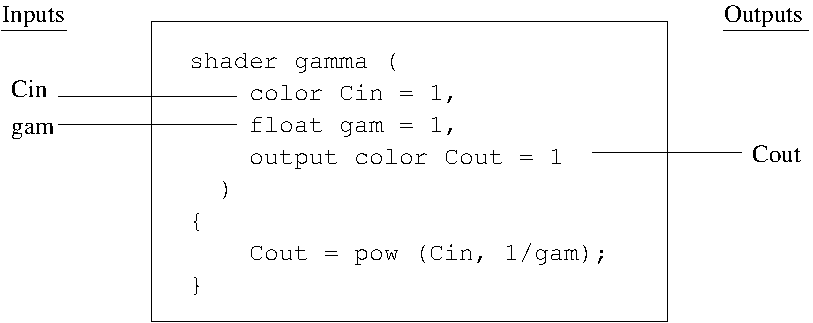
\includegraphics{Figures/shaderschematic}

\medskip

The shader's inputs and outputs are called \emph{shader parameters}.  
Parameters have default values, specified in the shader code, but may
also be given new values by the renderer at runtime.  

\subsection*{Shader instances}

A particular shader may be used many times in a scene, on different
objects or as different layers in a shader group.  Each separate use of
a shader is called a \emph{shader instance}.  Although all instances of
a shader are comprised of the same program code, each instance may
override any or all of its default parameter values with its own set of
\emph{instance values}.

Below is a
schematic showing a {\cf gamma} instance with the {\cf gam} parameter
overridden with an instance-specific value of {\cf 2.2}.

\bigskip

\bigspc\spc 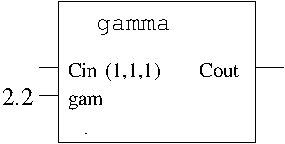
\includegraphics{Figures/instanceschematic}

\medskip



\subsection*{Shader groups and layers}

A \emph{shader group} is an ordered sequence of individual shaders
called \emph{layers} that are executed in turn.  Output parameters of an
earlier-executed layer may be \emph{connected} to an input parameter of
a later-executed layer.  This connected network of layers is sometimes
called a \emph{shader network} or a \emph{shader DAG} (directed acyclic
graph).  Of course, it is fine for the shader group to consist of a
single shader layer.

Below is a schematic showing how several shader instances may be
connected to form a shader group.

\bigskip

\noindent 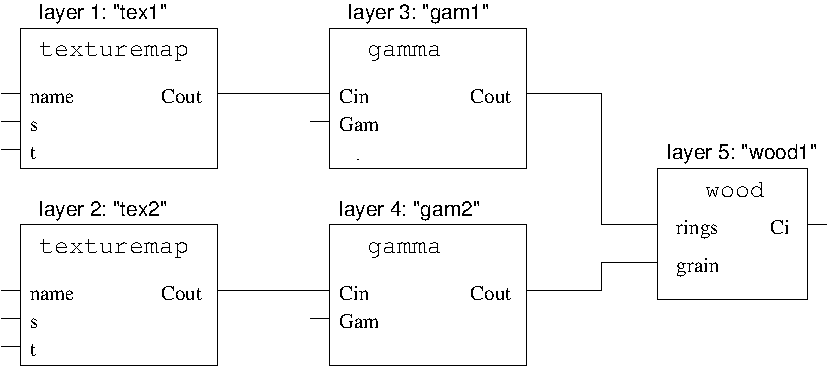
\includegraphics{Figures/groupschematic}

\bigskip

\noindent And here is sample pseudo-code shows how the above network may
be assembled using an API in the renderer\footnote{This document does
not dictate a specific renderer API for declaring shader instances,
groups, and connections; the code above is just an example of how
it might be done.}:

\begin{code}
    ShaderGroupBegin ()
    Shader ("texturemap",               /* shader name */
            "tex1",                     /* layer name */
            "string name", "rings.tx")  /* instance variable */
    Shader ("texturemap", "tex2", "string name", "grain.tx")
    Shader ("gamma", "gam1", "float gam", 2.2)
    Shader ("gamma", "gam2", "float gam", 1)
    Shader ("wood", "wood1")
    ConnectShaders ("tex1",     /* layer name A */
                    "Cout",     /* an output parameter of A */
                    "gam1",     /* layer name B */
                    "Cin")      /* Connect this layer of B to A's Cout */
    ConnectShaders ("tex2", "Cout", "gam2", "Cin")
    ConnectShaders ("gam1", "Cout", "wood1", "rings")
    ConnectShaders ("gam2", "Cout", "wood1", "grain")
    ShaderGroupEnd ()
\end{code}


\subsection*{Geometric primitives}

The \emph{scene} consists of primarily of geometric primitives,
light sources, and cameras.

\emph{Geometric primitives} are shapes such as NURBS, subdivision surfaces,
polygons, and curves.  The exact set of supported primitives may vary
from renderer to renderer.

Each geometric primitive carries around a set of named \emph{primitive
  variables}.  Nearly all shape types will have, among their primitive
variables, control point positions that, when interpolated, actually
designate the shape.  Some shapes will also allow the specification of
normals or other shape-specific data.  Arbitrary user data may also be
attached to a shape as primitive variables.  Primitive variables may be
interpolated in a variety of ways: one constant value per primitive, one
constant value per face, or per-vertex values that are interpolated
across faces in various ways.

If a shader input parameter's name and type match the name and type
of a primitive variable on the object (and that input parameters is
not already explicitly connected to another layer's output), the
interpolated primitive variable will override the instance value or
default.


\subsection*{Attribute state and shader assignments}

Every geometric primitive has a collection of \emph{attributes} (sometimes
called the \emph{graphics state}) that includes its transformation
matrix, the list of which lights illuminate it, whether it is one-sided
or two-sided, shader assignments, etc.  There may also be a long list of
renderer-specific or user-designated attributes associated with each
object.  A particular attribute state may be shared among many geometric
primitives.

The attribute state also includes shader assignments --- the shaders or
shader groups for each of several \emph{shader uses}, such as surface
shaders that designate how light reflects from each point on the shape,
displacement shaders that can add fine detail to the shape on a
point-by-point basis, volume shaders that describe how light is
scattered within a region of space, and light shaders that describe how
light is emitted from a light source.  A particular renderer may have
additional shader types that it supports.

%\subsection*{Shader types}
%
%There are several types of shaders: surface, displacement, light,
%volume.  The type of shader determines what it's allowed to do (for
%example, only displacement shaders can alter the surface position).
%There is also a generic kind of shader that can be used for any of the
%shader uses.

\subsection*{Shader execution state: parameter binding and global variables}

When the body of code of an individual shader is about to execute, all
its parameters are \emph{bound} --- that is, take on specific values
(from connections from other layers, interpolated primitive variables,
instance values, or defaults, in that order).

Certain state about the position on the surface where the shading is
being run is stored in so-called \emph{global variables}.  This includes
such useful data as the 3D coordinates of the point being shaded, the
surface normal and tangents at that point, etc.

Additionally, the shader may query other information about other
elements of the attribute state attached to the primitive, and
information about the renderer as a whole (rendering options, etc.).

\subsection*{Surface and volume shaders compute closures}

Surface shaders (and volume shaders) do not by themselves compute the
final color of light emanating from the surface (or along a volume).
Rather, the compute a \emph{closure}, which is a symbolic representation
describing the appearance of the surface, that may be more fully
evaluated later.  This is in effect a parameterized formula, in which
some inputs have definite numeric values, but others may depend on
quantities not yet known (such as the direction from which the surface
is being viewed, and the amount of light from each source that is
arriving at the surface).

For example, a surface shader may compute its result like this:

\begin{code}
    color paint = texture ("file.tx", u, v);
    Ci = paint * lambert (N);
\end{code}

\noindent In this example, the variable {\cf paint} will take on a
specific numeric value (by looking up from a texture map).  But the {\cf
  lambert()} function returns a \colorclosure, not a definite numeric
\color.  The output variable {\cf Ci} that represents the appearance of
the surface is also a \colorclosure, whose numeric value is not known
yet, except that it will be the product of {\cf paint} and a Lambertian
reflectance.

\bigskip

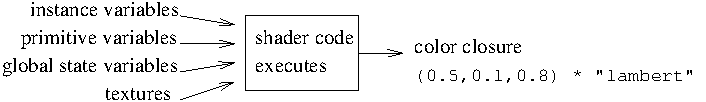
\includegraphics{Figures/shaderexecschematic}

\medskip

The closures output by surface and volume shaders can do a number of
interesting things that a mere number cannot:

\begin{itemize}
\item Evaluate: given input and output light directions, compute the
  proportion of light propagating from input to output.
\item Sample: given just an input (or output) direction, choose a
  scattering direction with a probability distribution that is
  proportional to the amount of light that will end up going in various
  directions.
\item Integrate: given all lights and a view direction, compute
  the total amount of light leaving the surface in the view direction.
\item Recompute: given changes only to lights (or only to one light),
  recompute the integrated result without recomputing other lights or
  any of the calculations that went into assembling constants in the
  closure (such as texture lookups, noise functions, etc.).
\end{itemize}

\begin{annotate}
At present, we are assuming that the primitive closure functions (such
as {\cf diffuse}, {\cf ward}, {\cf cooktorrance}, etc.) are all built
into the renderer, or implemented as renderer plugins.  At a later time,
possibly in a later draft or maybe not until a truly later version of
the spec, we will fully spec it out so that closure primitive functions
may be written in \langname.  But I fear that if we do it too soon,
we'll screw it up.  But, yes, the eventual goal is for you to be able to
write these primitive functions in the language itself.
\end{annotate}

\subsection*{Integrators}

The renderer contains a number of \emph{integrators} (selectable via the
renderer's API) which will combine the color closures computed by
surfaces and volumes with the light sources and view-dependent
information, to yield the amount of light visible to the camera.

\bigskip

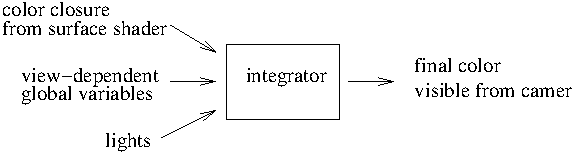
\includegraphics{Figures/integratorschematic}

\medskip

\begin{annotate}
At present, this document is written as if the integrators are built
into the renderer itself (or implemented as renderer plug-ins).  At a
later time, we intend to make it possible for integrators themselves
to be written in \langname.
\end{annotate}

\subsection*{Units}

You can tell the renderer (through a global option) what units the scene
is using for distance and time.  Then the shader has a built-in function
called {\cf transformu()} that works a lot like {\cf transform()}, but
instead of converting between coordinate systems, it converts among
units.  For example,

\begin{code}
    displacement bumpy (float bumpdist = 1,
                        string bumpunits = "cm")
    {
        // convert bumpdist to common units
        float spacing = transformu (bumpunits, "common", bumpdist);
        float n = noise (P / spacing);
        displace (n);
    }
\end{code}

So you can write a shader to achieve some effect in real world units,
and that shader is totally reusable on another show that used different
modeling units.

It knows all the standard names like \qkw{cm}, \qkw{in}, \qkw{km}",
etc., and can convert among any of those, as well as between named
coordinate systems.  For example,

\begin{code}
    float x = transformu ("object", "mm", 1);
\end{code}

now {\cf x} is the number of millimeters per unit of \objectspace on
that primitive.


\chapter{Lexical structure}
\label{chap:lexical}

\section{Characters}
\label{sec:lexical:chars}
\index{character set}

Source code for \langname consists of ASCII or UTF-8 characters.

The characters for space, tab, carriage return, and linefeed are
collectively referred to as \emph{whitespace}.  Whitespace characters
delimit identifiers, keywords, or other symbols, but other than that
have no syntactic meaning.  Multiple whitespace characters in a row
are equivalent to a single whitespace character. \index{whitespace}

Source code may be split into multiple lines, separated by end-of-line
markers (carriage return and/or linefeed).  Lines may be of any length
and end-of-line markers carry no significant difference from other 
whitespace, except that they terminate {\cf //} comments and delimit
preprocessor directives.

\section{Identifiers}
\label{sec:identifiers}
\index{identifiers}

\emph{Identifiers} are the names of variables, parameters, functions,
and shaders.  In \langname, identifiers consist of one or more
characters.  The first character may be a letter ({\cf A}-{\cf Z} or
{\cf a}-{\cf z}) or underscore (\verb|_|), and subsequent characters may
be letters, underscore, or numerals ({\cf 0}-{\cf 9}).  Examples of
valid and invalid identifiers are:

\begin{code}
    opacity       // valid
    Long_name42   // valid - letters, underscores, numbers are ok
    _foo          // valid - ok to start with an underscore

    2smart        // invalid - starts with a numeral
    bigbuck$      // invalid - $ is an illegal character
\end{code}


\section{Comments}
\label{sec:comments}
\index{comments}

\emph{Comments} are text that are for the human reader of programs, and
are ignored entirely by the \langname compiler.  Just like in C++, there
are two ways to designate comments in \langname:

\begin{enumerate}
\item Any text enclosed by {\cf /*} and {\cf */} will be considered
a comment, even if the comment spans several lines.

\begin{code}
    /* this is a comment */

    /* this is also
       a comment, spanning
       several lines */
\end{code}

\item Any text following {\cf //}, up to the end of the current line,
will be considered a comment.

\begin{code}
    // This is a comment
    a = 3;   // another comment
\end{code}
\end{enumerate}


\section{Keywords and reserved words}
\label{sec:lexical:keyreserved}

There are two sets of names that you may not use as identifiers:
keywords and reserved words.

The following are \emph{keywords} that have special meaning in
\langname: \index{keywords}

\begin{quote} {\cf

break closure color continue do else emit float for if illuminance
illuminate int matrix normal output point public return string struct
trace vector void while

}
\end{quote}

The following are \emph{reserved words} that currently have no special
meaning in \langname, but we reserve them for possible future use, or
because they are confusingly similar to keywords in related programming
languages: \index{reserved words}

\begin{quote} {\cf

bool case catch char class const delete default double 
enum extern false friend
goto inline long new operator private protected 
short signed sizeof static 
switch template this throw true try typedef 
uniform union unsigned varying virtual volatile

}
\end{quote}


\section{Preprocessor}
\label{sec:preprocessor}
\index{preprocessor} \index{C preprocessor|see{preprocessor}}
\indexapi{\#define}
\indexapi{\#undef}
\indexapi{\#if}
\indexapi{\#ifdef}
\indexapi{\#ifndef}
\indexapi{\#elif}
\indexapi{\#else}
\indexapi{\#endif}
\indexapi{\#include}

Shader source code is passed through a standard C preprocessor as a
first step in parsing.  

Preprocessor directives are designated by a hash mark ({\cf \#}) as the
first character on a line, followed by a preprocessor directive name.
Whitespace may optionally appear between the hash and the directive
name.

\langname compilers support the full complement of C/C++ preprocessing
directives, including:

\begin{code}
    #define
    #undef
    #if
    #ifdef
    #ifndef
    #elif
    #else
    #endif
    #include
\end{code}



\chapter{Gross syntax, shader types, parameters, functions}
\label{chap:grosssyntax}

The overall structure of a shader is as follows:
\medskip

\begin{quote}
\em
optional-function-or-struct-declarations \\

shader-type shader-name {\cf (} optional-parameters {\cf )} \\
\rm
{\cf \{ } \\
\em
\spc statements

{\cf \} }
\end{quote}

Note that \emph{statements} may include function or structure
definitions, local variable declarations, or public methods, as well as
ordinary execution instructions (such as assignments, etc.).

\section{Shader types}
\label{sec:shadertypes}
\index{shader types} \index{types!shader}

Shader types include the following: {\cf surface}, {\cf displacement},
{\cf light}, {\cf volume}, and generic {\cf shader}.  Some operations
may only be performed from within certain types of shaders (e.g., one
may only call {\cf displace()} or alter \P in a displacement shader),
and some global variables may only be accessed from within certain types
of shaders (e.g., {\cf dPdu} is not defined inside a volume shader).

Following are brief descriptions of the basic types of shaders:


\subsection*{{\cf surface} shaders}

Surface shaders determine the basic material properties of a surface and
how it reacts to light.  They are responsible for computing a
\colorclosure that describes the material, and optionally setting
other user-defined output variables.  They may not alter
the position of the surface.

Surface shaders are written as if they describe the behavior of a single
point on the primitive, and the renderer will choose the positions
surface at which the shader must be evaluated.

Surface shaders also are used to describe emissive objects, i.e., light
sources.  OSL does not need a separate shader type to describe lights.

\subsection*{{\cf displacement} shaders}

Displacement shaders alter the position and shading normal (or,
optionally, just the shading normal) to make a piece of geometry appear
deformed, wrinkled, or bumpy.  They are the only kind of shader that
is allowed to alter a primitive's position.

\subsection*{{\cf volume} shaders}

Volume shaders describe how a participating medium (air, smoke, glass,
etc.) reacts to light and affects the appearance of objects on the other
side of the medium.  They are similar to {\cf surface} shaders, except
that they may be called from positions that do not lie upon (and are not
necessarily associated with) any particular primitive.

\begin{comment}
\subsection*{{\cf light} shaders}

Light shaders describe how much energy a light source deposits at a
given destination.
\end{comment}


\subsection*{{\cf shader} generic shaders}

Generic shaders are used for utility code, generic routines that may be
called as individual layers in a shader group.  Generic shaders need not
specify a shader type, and therefore may be reused from inside surface,
displacement, or volume shader groups.  But as a result, they may
not contain any functionality that cannot be performed from inside all
shader types (for example, they may not alter \P, which can only be done
from within a displacement shader).


\section{Shader parameters}
\label{sec:shaderparams}
\index{shader parameters} \index{parameters!shader}

An individual shader has (optionally) many \emph{parameters} whose
values may be set in a number of ways so that a single shader may have
different behaviors or appearances when used on different objects.

\subsection{Shader parameter syntax}

Shader parameters are specified in the shader declaration, in
parentheses after the shader's name.  This is much like the parameters
to a \languagename function (or a function in C or similar languages),
except that shader parameters must have an \emph{initializer}, giving a
default value for the parameter.  Shader parameter default initializers
may be expressions (i.e., may be computed rather than restricted to
numeric constants), and are evaluated in the order that the parameters
are declared, and may include references to previously-declared
parameters.  Formally, the grammar for a simple parameter
declaration looks like this:

\medskip
\spc \emph{type parametername = default-expression} 
\medskip

\noindent where \emph{type} is one of the data types described
in Chapter~\ref{chap:types}, \emph{parametername} is the name of the
parameter, and \emph{default-expression} is a valid expression
(see Section~\ref{sec:expressions}).  Multiple parameters are 
simply separated by parentheses:

\medskip
\spc \emph{type1 ~ parameter1 = expr1} {\cf ,} \emph{type2 ~ parameter2 = expr2} {\cf ,} ...
\medskip


Fixed-length, one-dimensional array parameters are declared as follows:

\medskip
\spc \emph{type parametername} {\cf [ } \emph{array-length} {\cf ] = \{ } \emph{expr0}
  {\cf ,} \emph{expr1} ... {\cf \} }
\medskip

\noindent where \emph{array-length} is a positive integer constant
giving the length of the array, and the initializer is a series of
initializing expressions listed between curly braces.  The first
initializing expression provides the initializer for the first element
of the array, the second expression provides the initializer for the
second element of the array, and so on.  If the number of initializing
expressions is less than the length of the array, any additional array
elements will have undefined values.

Arrays may also be declared without a set length:

\medskip
\spc \emph{type parametername} {\cf [ ] = \{ } \emph{expr0}
  {\cf ,} \emph{expr1} ... {\cf \} }
\medskip

\noindent where no array length is found between the square brackets.
This indicates that the array's length will be determined based on
whatever is passed in --- a connection from the output of another shader
in the group (take on the length of that output), an instance value
(take on the length specified by the declaration of the instance value),
or a primitive variable (length determined by its declaration on the
primitive).  If no instance value, primitive value, or connection is
supplied, then the number of initializing expressions will determine the
length, as well as the default values, of the array.

Structure parameters are also straightforward to declare:

\medskip
\spc \emph{structure-type parametername} {\cf = \{ } \emph{expr0}
  {\cf ,} \emph{expr1} ... {\cf \} }
\medskip

\noindent where \emph{structure-type} is the name of a
previously-declared {\cf struct} type, and the \emph{expr} initializers
correspond to each respective field within the structure.  An
initializer of appropriate type is required for every field of the
structure.

\subsection{Shader output parameters}
\index{shader output parameters} \index{output parameters!shader}

Shader parameters are, by default, read-only in the body of the
shader.  However, special \emph{output parameters} may be altered
by execution of the shader.  Parameters may be designated outputs
by use of the {\cf output} keyword immediately prior to the
type declaration of the parameter:

\medskip
\spc {\cf output} \emph{type parametername} {\cf = } \emph{expr}
\medskip

\noindent (Output parameters may be arrays and structures, but we will
omit spelling out the obvious syntax here.)

Output parameters may be connected to inputs of later-run shader layers
in the shader group, may be queried by later-run shaders in the group
via message passing (i.e., {\cf getmessage()} calls), or used by the
renderer as an output image channel (in a manner described through the
renderer's API).

\subsection{Shader parameter example}

Here is an example of a shader declaration, with several parameters:

\begin{code}
    surface wood ( 
               /* Simple params with constant initializers */
                   float Kd = 0.5,
                   color woodcolor = color (.7, .5, .3),
                   string texturename = "wood.tx",
               /* Computed from an earlier parameter */
                   color ringcolor = 0.25 * woodcolor,
               /* Fixed-length array */
                   color paintcolors[3] = { color(0,.25,0.7), color(1,1,1),
                                            color(0.75,0.5,0.2) },
               /* variable-length array */
                   int pattern[] = { 2, 4, 2, 1 },
               /* output parameter */
                   output color Cunlit = 0
                 )
    {
       ...
    }
\end{code}

\subsection{How shader parameters get their values}

Shader parameters get their values in the following manner,
in order of decreasing priority:

\begin{itemize}
\item If the parameter has been designated by the renderer to be
  connected to an output parameter of a previously-executed shader layer
  within the shader group, that is the value it will get.
\item If the parameter matches the name and type of a per-primitive,
  per-face, or per-vertex \emph{primitive variable} on the particular
  piece of geometry being shaded, the parameter's value will be computed
  by interpolating the primitive variable for each position that must be
  shaded.
\item If there is no connection or primitive variable, the parameter may
  will take on an \emph{instance value}, if that parameter was given an
  explicit per-instance value at the time that the renderer referenced
  the shader (associating it with an object or set of objects).
\item If none of these overrides is present, the parameter's value will
  be determined by executing the parameter initialization code in the
  shader.
\end{itemize}

This triage is performed per parameter, in order of declaration.  So,
for example, in the code sample above where the default value for {\cf
  ringcolor} is a scaled version of {\cf woodcolor}, this relationship
would hold whether {\cf woodcolor} was the default, an instance value,
an interpolated primitive value, or was connected to another layer's
output.  Unless {\cf ringcolor} itself was given an instance, primitive,
or connection value, in which case that's what would be used.



\section{Shader metadata}
\label{sec:metadata}
\index{metadata} \index{shader metadata}

A shader may optionally include \emph{metadata} (data \emph{about} the
shader, as opposed to data \emph{used by} the shader).  Metadata may be
used to annotate the shader or any of its individual parameters with
additional hints or information that will be compiled into the shader
and may be queried by applications.  A common use of metadata is to
specify user interface hints about shader parameters --- for example,
that a particular parameter should only take on integer values, should
have an on/off checkbox, is intended to be a filename, etc.

Metadata is specified inside double brackets {\cf [[} and {\cf ]]}
enclosing a comma-separated list of metadata items.  Each metadatum
looks like a parameter declaration --- having a data type, name, and
initializer.  However, metadata may only be simple types (not arrays or
closures) and their value initializers must be numeric or string
constants (not computed expression).

Metadata about the shader as a whole is placed between the shader name
and the parameter list.  Metadata about shader parameters are placed
immediately after the parameter's initializing expression, but before
the comma or closing parentheses that terminates the parameter
description.

Below is an example shader declaration showing the use of shader and
parameter metadata:

\begin{code}
    surface wood 
                [[ string description = "Realistic wood shader" ]]
        ( 
           float Kd = 0.5
               [[ string description = "Diffuse reflectivity",
                  float UImin = 0, float UImax = 1 ]] ,
           color woodcolor = color (.7, .5, .3)
               [[ string description = "Base color of the wood" ]],
           color ringcolor = 0.25 * woodcolor
               [[ string description = "Color of the dark rings" ]],
           string texturename = "wood.tx"
               [[ string description = "Texture map for the grain",
                  string UItype = "filename" ]]
        )
    {
       ...
    }
\end{code}

The metadata are not semantically meaningful; that is, the metadata does
not affect the actual execution of the shader.  Most metadata exist only
to be embedded in the compiled shader and able to be queried by other
applications, such as to construct user interfaces for shader assignment
that allow usage tips, appropriate kinds of widgets for setting each
parameter, etc.  

The choice of metadata and their meaning is completely up to the shader
writer and/or modeling system.  However, we propose some conventions
below.  These conventions are not intended to be comprehensive, nor to
meet all your needs --- merely to establish a common nomenclature for
the most common metadata uses.

\apiitem{string description}
Describes the purpose and use of the shader or parameter.
\apiend

\apiitem{string URL}
Provides a URL for full documentation of the shader or parameter.
\apiend

\apiitem{string units}
Gives the assumed units, if any, for the parameter (e.g., \qkw{cm},
\qkw{sec}, \qkw{degrees}).
The compiler or renderer may issue a warning if it detects that this
assumption is being violated (for example, the compiler can warn
if a \qkw{degrees} variable is passed as the argument to {\cf cos}).
\apiend

\apiitem{int normalized}
For a \vector or \normal, a nonzero value is a hint that the shader
expects the vector to be unit length.  The renderer may use this hint to
print a warning if the parameter or value is not of unit length, and the
compiler may warn if a \qkw{normalized} variable is assigned a non-unit
value.
\apiend

\apiitem{string UIlabel}
A short label to be displayed in the UI for this parameter.  If not
present, the parameter name itself should be used as the widget label.
\apiend

\apiitem{float UImin \\ float UImax}
Minimum and maximum values for a parameter that should never be
exceeded.  If either the minimum or maximum is not present, valid values
for the parameter are assumed to be unbounded in one or both directions.
(For an {\cf int} parameter, the {\cf UImin} and/or {\cf UImax} should
also be declared as an {\cf int}.)
\apiend

\apiitem{float UIsoftmin \\ float UIsoftmax}
``Soft'' minimum and maximum value for a \float parameter, that is, a
default range for presentation in the UI, but which may be overridden by
the user. (For an {\cf int} parameter, the {\cf UIsoftmin} and/or {\cf
  UIsoftmax} should also be declared as an {\cf int}.)
\apiend

\apiitem{float UIstep}
The suggested step size for incrementing or decrementing the value
(within the appropriate min/max range).
\apiend

\apiitem{string UIenabler}
The name of another parameter that, only if nonzero (or the
non-empty string) unlocks adjustment of this parameter.  For example,
a parameter called \qkw{Kr} (reflectivity) may be en enabler for
the \qkw{reflectionblur} parameter; zero reflectivity would gray-out
the blur controls, which would be ignored if there were no reflection.
\apiend

\apiitem{float UIseparator}
If nonzero, hints that the application's GUI should draw a visual 
separator immediately before this parameter.
\apiend

\apiitem{string UIgroupbegin \\ string UIgroupend}
Denote the first and last parameters of a set of related parameters, as a
hint that an application may wish to label or visually separate a
collection of parameters.  The string value should be the name or brief
description of the group.
\apiend

\apiitem{string UItype} 
Provides a hint about exactly what kind of UI widget is appropriate for
the given parameter (if not the obvious default, such as a slider for a
\float parameter, or a color picker for a \color parameter).  Recommended
values include:

\vspace{-12pt}
\begin{description}
\item[] \spc
\item[\rm \halfspc ~ \qkw{bool}] Indicates that a \float or {\cf int}
  parameter should only take on a 0 or 1 value, and therefore a checkbox
  may be a more appropriate UI widget.
\item[\rm \qkw{string}] Indicates that the appropriate UI widget is a text
  input box (default for string parameters).  A smart UI may also allow
  a file selection dialog, since most strings (but not all) are used
  for texture names.
\item[\rm \qkw{texture}] Indicates a string variable whose value will be
  used as the name of a texture map.  An appropriate GUI widget might
  be a file selection dialog.
\item[\rm \qkw{environment}] Indicates a string variable whose value may
  either be an environment map or the name of a geometry set.  An
  appropriate GUI widget might be a combination file selection and
  pull-down menu of known geometry set names.
\item[\rm \qkw{shadow}] Indicates a string variable whose value may
  either be a shadow map or the name of a geometry set.
\item[\rm \qkw{geometryset}] Indicates a string variable whose value must
  be a geometry set.  An appropriate GUI widget may be a pull-down
  menu of known geometry sets.
\item[\rm \qkw{coordsys}] Indicates a string variable whose value will be
  used as a coordinate system name.  An appropriate GUI widget may be
  a pull-down menu of known coordinate systems.
\item[\rm \qkw{enum:label0,label1,...}] Indicates that the appropriate UI
  widget is a pulldown menu that selects among the strings \qkw{label0},
  \qkw{label1}, and so on.
  If the shader parameter is a {\cf string}, the selected label should be
  passed as the shader parameter value.  If the shader parameter is an
  \inttype, the selected label should indicate that the value passed
  should be 0, 1, 2, ..., the index of the selected label.
  Labels may be associated with \float or {\cf int} values other than
  their indices using the following syntax:
  \begin{code}
    float frequency = 0.5
        [[ string UItype = "enum:low=0.2,medium=0.5,high=0.9" ]]
    int pattern = 0
        [[ string UItype = "enum:oak=0,elm=1,walnut=2" ]]
  \end{code}
\end{description}
\apiend

The use of metadata is entirely optional on the part of the shader
writer, and any application that queries shader metadata is free to
honor or ignore any metadata it finds.


\newpage
\section{Functions}
\label{sec:functions}
\index{functions!declarations}

You may define functions much like in C or C++.

\begin{quote}
\em
return-type ~ function-name ~ {\rm\cf (} optional-parameters {\rm\cf )} \\
\rm
{\cf \{ } \\
\em
\spc statements

{\cf \} }
\end{quote}

Parameters to functions are similar to shader parameters, except that
they do not permit initializers.  A function call must pass values for
all formal parameters.  Function parameters in \langname are all
\emph{passed by reference}, and are read-only within the body of the
function unless they are also designated as {\cf output} (in the same
manner as output shader parameters).

Like for shaders, statements inside functions may be actual executions
(assignments, function call, etc.), local variable declarations (visible
only from within the body of the function), or local function
declarations (callable only from within the body of the function).

The return type may be any simple data type, a {\cf struct}, or a {\cf
  closure}.  Functions may not return arrays.  The return type may be
{\cf void}, indicating that the function does not return a value (and
should not contain a {\cf return} statement).  A {\cf return} statement
inside the body of the function will halt execution of the function at
that point, and designates the value that will be returned (if not a
{\cf void} function).

Functions may be \emph{overloaded}.  That is, multiple functions may be
defined to have the same name, as long as they have differently-typed
parameters, so that when the function is called the list of arguments
can disambiguate which version of the function is desired.

\section{Public methods}
\label{sec:publicmethods}
\indexapi{public}
\index{public methods}

Ordinary (non-public) functions inside a shader may be called only from
within the shader; they do not generate entry points that the renderer
is aware of.

A \emph{public method} is a function that may be directly called by the
renderer.  Only top-level local functions of a shader --- that is,
declared within the braces that define the local scope of the shader,
but not within any other such function --- may be public methods.  A
function may be designated a public method by using the {\cf public}
keyword immediately before the function declaration:

\begin{quote}
\em shader-type shader-name ( params ) \\
{\rm\cf \{}

\spc {\rm\cf public} \em ~ return-type ~ function-name ~ {\rm \cf (}
optional-parameters {\rm \cf )} \\
\spc {\rm \cf \{ } \\
\spc\spc statements \\
\spc {\rm \cf \} } \\

\spc ...\\
{\rm\cf \}}
\end{quote}


\begin{annotate}
A given renderer will publish a list of public methods (names, arguments
expected, and return value) that has particular meaning for that
renderer.  For example, a renderer may honor a public method
\begin{code}
    public float maxdisplacement ()
\end{code}
\noindent that computes and returns the maximum distance 
that a displacement shader will move any surface points.

At some later point, this spec will recommend several ``standard''
public methods that should be honored by most renderers.
\end{annotate}

\chapter{Data types}
\label{chap:types}
\index{types|(}

\langname provides several built-in simple data types for performing
computations inside your shader:
\smallskip

\noindent\begin{tabular}{|p{0.75in}|p{4.75in}|}
\hline
{\cf int}	& Integer data \\[1ex]
%\hline
{\cf float}	& Scalar floating-point data (numbers) \\[1ex]
%\hline
{\cf point
vector
normal}		& Three-dimensional positions, directions, and surface
		  orientations \\[7ex]
%\hline
{\cf color}	& Spectral reflectivities and light energy values \\[1ex]
%\hline
{\cf matrix}	& $4 \times 4$ transformation matrices \\[1ex]
%\hline
{\cf string}	& Character strings (such as filenames) \\[1ex]
{\cf void}      & Indicates functions that do not return a value \\[1ex]
\hline
\end{tabular}

In addition, you may create arrays and structures (much like C), and
\langname has a new type of data structure called a \emph{closure}.

The remainder of this chapter will describe the simple and aggregate
data types available in \langname.

\section{{\cf int}}
\label{sec:types:int}
\indexapi{int} \index{types!{\cf int}}

The basic type for discrete numeric values is {\cf int}.  The size of
the {\cf int} type is renderer-dependent, but is guaranteed to be at
least 32 bits.

Integer constants are constructed the same way as in C.  The following
are examples of {\cf int} constants: {\cf 1}, {\cf -32}, etc.

Unlike C, no unsigned, bool, char, short, or long types are supplied.
This is to simplify the process of writing shaders (as well as
implementing shading systems).

The following operators may be used with \inttype values (in order of
decreasing precedence, with each box holding operators of the same
precedence):

\smallskip

\noindent \begin{tabular}{|p{1in}|p{0.5in}|p{3.75in}|}
operation & result & ~ \\
\hline
\inttype\ {\ce ++} & \inttype & post-increment by 1 \\[0.5ex]
\inttype\ {\ce --} & \inttype & post-decrement by 1 \\[0.5ex]
\hline
{\ce ++} \inttype & \inttype & pre-increment by 1 \\[0.5ex]
{\ce --} \inttype & \inttype & pre-decrement by 1 \\[0.5ex]
{\cf {\bfseries -} int} & \inttype & unary negation \\[0.5ex]
\verb|~| {\cf int} & \inttype & bitwise complement (1 and 0 bits flipped) \\[0.5ex]
{\cf {\bfseries !} int} & \inttype & boolean `not' (1 if operand is zero, otherwise 0) \\[0.5ex]
\hline
{\cf int {\bfseries *} int} & \inttype & multiplication \\[0.5ex]
{\cf int {\bfseries /} int} & \inttype & division \\[0.5ex]
{\cf int {\bfseries \%} int} & \inttype & modulus \\[0.5ex]
\hline
{\cf int {\bfseries +} int} & \inttype & addition \\[0.5ex]
{\cf int {\bfseries -} int} & \inttype & subtraction \\[0.5ex]
\hline
{\cf int {\bfseries <<} int} & \inttype & shift left \\[0.5ex]
{\cf int {\bfseries >>} int} & \inttype & shift right \\[0.5ex]
\hline
{\cf int {\bfseries <} int} & \inttype & 1 if the first value is less
than the second, else 0 \\[0.5ex]
{\cf int {\bfseries <=} int} & \inttype & 1 if the first value is less
or equal to the second, else 0 \\[0.5ex]
{\cf int {\bfseries >} int} & \inttype &  1 if the first value is
greater than the second, else 0 \\[0.5ex]
{\cf int {\bfseries >=} int} & \inttype & 1 if the first value is
greater than or equal to the second, else 0 \\[0.5ex]
\hline
{\cf int {\bfseries ==} int} & \inttype & 1 if the two values are equal,
else 0 \\[0.5ex]
{\cf int {\bfseries !=} int} & \inttype & 1 if the two values are different,
else 0 \\[0.5ex]
\hline
{\cf int {\bfseries \&} int} & \inttype & bitwise and \\[0.5ex]
\hline
{\cf int {\bfseries \verb|^|} int} & \inttype & bitwise exclusive or \\[0.5ex]
\hline
{\cf int {\bfseries |} int} & \inttype & bitwise or \\[0.5ex]
\hline
{\cf int {\bfseries \&\&} int} & \inttype & boolean and (1 if both operands are
nonzero, otherwise 0) \\[0.5ex]
\hline
{\cf int {\bfseries ||} int} & \inttype & boolean or (1 if either operand is
nonzero, otherwise 0) \\[0.5ex]
\hline
\end{tabular}



\section{{\cf float}}
\label{sec:types:float}
\indexapi{float} \index{types!{\cf float}}

The basic type for scalar floating-point numeric values is \float.  The
size of the {\cf float} type is renderer-dependent, but is guaranteed to
be at least IEEE 32-bit float (the standard C \float data type).
Individual renderer implementations may choose to implement \float with
even more precision (such as using the C {\cf double} as the underlying
representation).

Floating-point constants are constructed the same way as in C.
The following are examples of {\cf float} constants:  {\cf 1.0},
{\cf 2.48}, {\cf -4.3e2}.

An \inttype may be used in place of a \float when used with any valid
\float operator.  In such cases, the \inttype will be promoted to a
\float and the resulting expression will be \float.  An \inttype may
also be passed to a function that expects a \float parameters, with the
\inttype automatically promoted to \float.

The following operators may be used with \float values (in order of
decreasing precedence, with each box holding operators of the same
precedence):

\medskip

\noindent \begin{tabular}{|p{1.25in}|p{0.5in}|p{3.5in}|}
operation & result & ~ \\
\hline
\float\ {\ce ++} & \float & post-increment by 1 \\[0.5ex]
\float\ {\ce --} & \float & post-decrement by 1 \\[0.5ex]
\hline
{\ce ++} \float & \float & pre-increment by 1 \\[0.5ex]
{\ce --} \float & \float & pre-decrement by 1 \\[0.5ex]
{\cf {\bfseries -} float} & \float & unary negation \\[0.5ex]
\hline
{\cf float {\bfseries *} float} & \float & multiplication \\[0.5ex]
{\cf float {\bfseries /} float} & \float & division \\[0.5ex]
\hline
{\cf float {\bfseries +} float} & \float & addition \\[0.5ex]
{\cf float {\bfseries -} float} & \float & subtraction \\[0.5ex]
\hline
{\cf float {\bfseries <} float} & \inttype & 1 if the first value is less
than the second, else 0 \\[0.5ex]
{\cf float {\bfseries <=} float} & \inttype & 1 if the first value is less
or equal to the second, else 0 \\[0.5ex]
{\cf float {\bfseries >} float} & \inttype &  1 if the first value is
greater than the second, else 0 \\[0.5ex]
{\cf float {\bfseries >=} float} & \inttype & 1 if the first value is
greater than or equal to the second, else 0 \\[0.5ex]
\hline
{\cf float {\bfseries ==} float} & \inttype & 1 if the two values are equal,
else 0 \\[0.5ex]
{\cf float {\bfseries !=} float} & \inttype & 1 if the two values are different,
else 0 \\[0.5ex]
\hline
\end{tabular}



\section{{\cf color}}
\label{sec:types:color}
\indexapi{color} \index{types!{\cf color}}

The \color type is used to represent 3-component (RGB) spectral
reflectivities and light energies.  You can assemble a
color out of three floats, either representing an RGB triple or some
other color space known to the renderer, as well as from a single
float (replicated for all three channels).  Following are some examples:

\begin{code}
    color (0, 0, 0)              // black
    color ("rgb", .75, .5, .5)   // pinkish
    color ("hsv", .2, .5, .63)   // specify in "hsv" space
    color (0.5)                  // same as color (0.5, 0.5, 0.5)
\end{code}

All these expressions above return colors in \rgbspace.  Even
the third example returns a color in \rgbspace\ --- specifically, the
RGB value of the color that is equivalent to hue 0.2, saturation 0.5,
and value 0.63.  In other words, when assembling a color from components
given relative to a specific color space in this manner, there is an
implied transformation to \rgbspace.  Table~\ref{tab:colorspacenames}
lists the built-in color spaces.

\begin{table}[htbp]
\caption{Names of color spaces.}\label{tab:colorspacenames}
\begin{tabular}{|p{0.7in}|p{4.7in}|}
\hline
{\cf "rgb"} & The coordinate system that all colors start out in, and
in which the renderer expects to find colors that are set by
your shader.   \\
\hline 
{\cf "hsv"} & hue, saturation, and value. \\
\hline 
{\cf "hsl"} & hue, saturation, and lightness. \\
\hline 
{\cf "YIQ"} & the color space used for the NTSC television standard. \\
\hline 
{\cf "xyz"} & CIE \emph{XYZ} coordinates. \\
\hline 
{\cf "xyY"} & CIE \emph{xyY} coordinates. \\
\hline 
\end{tabular}
\end{table}

Colors may be assigned another color or a \float value (which sets
all three components to the value).  For example:

\begin{code}
    color C;
    C = color (0, 0.3, 0.3);
    C = 0.5;                    // same as C = color (0.5, 0.5, 0.5)
\end{code}

Colors can have their individual components examined and set using the
{\cf []} array access notation.  For example:

\begin{code}
    color C;
    float g = C[1];   // get the green component
    C[0] = 0.5;       // set the red component
\end{code}

\noindent Components 0, 1, and 2 are red, green, and blue, respectively.
It is an error to access a color component with an index outside the
$[0...2]$ range.

The following operators may be used with \color values (in order of
decreasing precedence, with each box holding operators of the same
precedence):

\medskip

\noindent \begin{tabular}{|p{1.5in}|p{0.5in}|p{3.25in}|}
operation & result & ~ \\
\hline
\color\ {\ce [} \inttype {\ce ]} & \float & component access \\[0.5ex]
\hline
{\ce -} \color & \color & unary negation \\[0.5ex]
\hline
\color\ {\ce *} \color & \color & component-wise multiplication \\[0.5ex]
\color\ {\ce *} \float & \color & scaling \\[0.5ex]
\float\ {\ce *} \color & \color & scaling \\[0.5ex]
\color\ {\ce /} \color & \color & component-wise division \\[0.5ex]
\color\ {\ce /} \float & \color & scaling \\[0.5ex]
\float\ {\ce /} \color & \color & scaling \\[0.5ex]
\hline
\color\ {\ce +} \color & \color & component-wise addition \\[0.5ex]
\color\ {\ce -} \color & \color & component-wise subtraction \\[0.5ex]
\hline
\color\ {\ce ==} \color & \inttype & 1 if the two values are equal,
else 0 \\[0.5ex]
\color\ {\ce !=} \color & \inttype & 1 if the two values are different,
else 0 \\[0.5ex]
\hline
\end{tabular}

All of the binary operators may combine a scalar value (\float or
\inttype) with a \color, treating the scalar if it were a \color with
three identical components.


\section{Point-like types: {\cf point}, {\cf vector}, {\cf normal}}
\label{sec:types:point}
\indexapi{point} \indexapi{vector} \indexapi{normal}
\index{types!{\cf point}} \index{types!{\cf vector}} \index{types!{\cf normal}}

Points, vectors, and normals are similar data types with identical
structures but subtly different semantics.  We will frequently refer to
them collectively as the ``point-like'' data types when making
statements that apply to all three types.

A \point is a position in 3D space.  A \vector has a length and
direction, but does not exist in a particular location.  A \normal is a
special type of vector that is \emph{perpendicular} to a surface, and
thus describes the surface's orientation.  Such a perpendicular vector
uses different transformation rules than ordinary vectors, as we will
describe below.

All of these point-like types are internally represented by three
floating-point numbers that uniquely describe a position or
direction relative to the three axes of some coordinate system.  

All points, vectors, and normals are described relative to some
coordinate system.  All data provided to a shader (surface information,
graphics state, parameters, and vertex data) are relative to one
particular coordinate system that we call the {\cf "common"} coordinate
system.  The {\cf "common"} coordinate system is one that is convenient
for the renderer's shading calculations.
\label{sect:commonspace}

You can ``assemble'' a point-like type out of three floats using a
constructor:

\begin{code}
        point (0, 2.3, 1)
        vector (a, b, c)
        normal (0, 0, 1)
\end{code}

\noindent These expressions are interpreted as a point, vector, and normal
whose three components are the floats given, relative to \commonspace\ .

As with colors, you may also specify the coordinates relative to some other
coordinate system:

\begin{code}
    Q = point ("object", 0, 0, 0);
\end{code}

This example assigns to {\cf Q} the point at the origin of
\objectspace.  However, this statement does \emph{not} set the
components of {\cf Q} to (0,0,0)!  Rather, {\cf Q} will contain the
\commonspace\ coordinates of the point that is at the same location as
the origin of \objectspace.  In other words, the point constructor that
specifies a space name implicitly specifies a transformation
to \commonspace.  This type of constructor also can be used for vectors
and normals.

The choice of \commonspace is renderer-dependent, though will usually
be equivalent to either \cameraspace or \worldspace.

Some computations may be easier in a coordinate system other than
\currentspace.  For example, it is much more convenient to apply a
``solid texture'' to a moving object in its \objectspace than in
\currentspace.  For these reasons, SL provides a built-in 
{\cf transform} function that
allows you to transform points, vectors, and normals 
among different coordinate systems (see Section~\ref{sec:stdlib:geom}).  Note,
however, that \langname does not keep track of which point variables are
in which coordinate systems.  It is the responsibility of the shader
programmer to keep track of this and ensure that, for example, lighting
computations are performed using quantities in \commonspace.

Several coordinate systems are predefined by name, listed in
Table~\ref{tab:spacenames}.  Additionally, a renderer will probably
allow for additional coordinate systems to be named in the scene
description, and these names may also be referenced inside your shader
to designate transformations.

\begin{table}[htbp]
\caption{Names of predeclared geometric spaces.\label{tab:spacenames}}
\begin{tabular}{|p{0.7in}|p{4.7in}|}
\hline
{\cf "common"} & The coordinate system that all spatial values start out in and
the one in which all lighting calculations are carried out.  Note that
the choice of {\cf "common"} space may be different on each renderer. \\
\hline 
{\cf "object"} & The local coordinate system of the graphics primitive (sphere,
patch, etc.) that we are shading. \\
\hline 
{\cf "shader"} & The local coordinate system active at the time that the shader
was instanced. \\
\hline 
{\cf "world"} & The world coordinate system designated in the scene. \\
\hline 
{\cf "camera"} & The coordinate system with its origin at the center of
the camera lens, $x$-axis pointing right, $y$-axis pointing up, and
$z$-axis pointing into the screen. \\
\hline 
{\cf "screen"} & The coordinate system of the camera's image plane
(after perspective transformation, if any).  Coordinate (0,0) of {\cf
"screen"} space is looking along the $z$-axis of \cameraspace. \\
\hline 
{\cf "raster"} & 2D pixel coordinates, with (0,0) as the upper-left
corner of the image and (xres, yres) as the lower-right corner. \\
\hline 
{\cf "NDC"} & 2D Normalized Device Coordinates --- like raster space, but
normalized so that $x$ and $y$ both run from 0 to 1 across the whole
image, with (0,0) being at the upper left of the image, and (1,1) being
at the lower right. \\
\hline 
\end{tabular}
\end{table}

Point types can have their individual components examined and set using
the {\cf []} array access notation.  For example:

\begin{code}
    point P;
    float y = P[1];   // get the y component
    P[0] = 0.5;       // set the x component
\end{code}

\noindent Components 0, 1, and 2 are $x$, $y$, and $z$, respectively.
It is an error to access a point component with an index outside the
$[0...2]$ range.

The following operators may be used with point-like values (in order of
decreasing precedence, with each box holding operators of the same
precedence):

\medskip

\noindent \begin{tabular}{|p{1.5in}|p{0.5in}|p{3.25in}|}
operation & result & ~ \\
\hline
\emph{ptype}\ {\ce [} \inttype {\ce ]} & \float & component access \\[0.5ex]
\hline
{\ce -} \emph{ptype} & \vector & component-wise unary negation \\[0.5ex]
\hline
\emph{ptype}\ {\ce *} \emph{ptype} & \emph{ptype} & component-wise multiplication \\[0.5ex]
\float\ {\ce *} \emph{ptype} & \emph{ptype} & scaling of all components \\[0.5ex]
\emph{ptype}\ {\ce *} \float & \emph{ptype} & scaling of all components \\[0.5ex]
\emph{ptype}\ {\ce /} \emph{ptype} & \emph{ptype} & component-wise division \\[0.5ex]
\emph{ptype}\ {\ce /} \float & \emph{ptype} & division of all components \\[0.5ex]
\float\ {\ce /} \emph{ptype} & \emph{ptype} & division by all components \\[0.5ex]
\hline
\emph{ptype}\ {\ce +} \emph{ptype} & \emph{ptype} & component-wise addition \\[0.5ex]
\emph{ptype}\ {\ce -} \emph{ptype} & \vector & component-wise subtraction \\[0.5ex]
\hline
\emph{ptype}\ {\ce ==} \emph{ptype} & \inttype & 1 if the two values are equal,
else 0 \\[0.5ex]
\emph{ptype}\ {\ce !=} \emph{ptype} & \inttype & 1 if the two values are different,
else 0 \\[0.5ex]
\hline
\end{tabular}

\smallskip

\noindent The generic \emph{ptype} is listed in places where any
of \point, \vector, or \normal may be used.

All of the binary operators may combine a scalar value (\float or
\inttype) with a point-like type, treating the scalar if it were
point-like with three identical components.


\section{{\cf matrix}}
\label{sec:types:matrix}
\indexapi{matrix} \index{types!{\cf matrix}}

\langname has a \matrix type that represents the transformation matrix
required to transform points and vectors between one coordinate system
and another.  Matrices are represented internally by 16 floats (a $4
\times 4$ homogeneous transformation matrix).

A \matrix can be constructed from a single float or 16 floats.  For
example:

\begin{code}
    matrix zero = 0;   // makes a matrix with all 0 components
    matrix ident = 1;  // makes the identity matrix

    // Construct a matrix from 16 floats
    matrix m = matrix (m00, m01, m02, m03, m10, m11, m12, m13, 
                       m20, m21, m22, m23, m30, m31, m32, m33);
\end{code}

\noindent Assigning a single floating-point number $x$ to a matrix will result
in a matrix with diagonal components all being $x$ and other
components being zero (i.e., $x$ times the identity matrix).
Constructing a matrix with 16 floats will create the matrix whose
components are those floats, in row-major order.  

Similar to point-like types, a {\cf matrix} may be constructed in
reference to a named space:

\begin{code}
    // Construct matrices relative to something other than "common"
    matrix q = matrix ("shader", 1);
    matrix m = matrix ("world", m00, m01, m02, m03, m10, m11, m12, m13, 
                               m20, m21, m22, m23, m30, m31, m32, m33);
\end{code}

\noindent The first form creates the matrix that transforms points from
\currentspace to \shaderspace.  Transforming points by this matrix
is identical to calling {\cf transform("shader",...)}.
The second form prepends the current-to-world transformation matrix
onto the $4 \times 4$ matrix with components $m_{0,0} ... m_{3,3}$.
Note that although we have used {\cf "shader"} and {\cf "world"}
space in our examples, any named space is acceptable.

A matrix may also be constructed from the names of two coordinate
systems, yielding the matrix that transforms coordinates from the
first named space to the second named space:

\begin{code}
    matrix m = matrix ("object", "world");
\end{code}

\noindent The example returns the \emph{object-to-world} transformation
matrix.

Matrix variables can be tested for equality and inequality with the
{\cf ==} and {\cf !=} boolean operators.  Also, the {\cf *} operator
between matrices denotes matrix multiplication, while {\cf m1 / m2}
denotes multiplying {\cf m1} by the inverse of matrix {\cf m2}.  Thus,
a matrix can be inverted by writing {\cf 1/m}.  In addition, some
functions will accept matrix variables as arguments, as described in
Section~\ref{chap:stdlibrary}.

Individual components of a matrix variable may be set or accessed
using array notation, for example,

\begin{code}
    matrix M;
    float x = M[row][col];
    M[row][col] = 1;
\end{code}

Valid component indices are integers on $[0...3]$.  It is an error to
access a matrix component with either a row or column outside this
range.

The following operators may be used with matrices (in order of
decreasing precedence, with each box holding operators of the same
precedence):

\medskip
\noindent \begin{tabular}{|p{1.5in}|p{0.5in}|p{3.25in}|}
operation & result & ~ \\
\hline
\matrix\ {\ce [} \inttype {\ce ][} \inttype {\ce ]} & \float & component
access (row, column) \\[0.5ex]
\hline
{\ce -} \matrix & \matrix & unary negation \\[0.5ex]
\hline
\matrix\ {\ce *} \matrix & \matrix & matrix multiplication \\[0.5ex]
\matrix\ {\ce *} \float & \matrix & component-wise scaling \\[0.5ex]
\float\ {\ce *} \matrix & \matrix & component-wise scaling \\[0.5ex]
\matrix\ {\ce /} \matrix & \matrix & multiply the first matrix by the
\emph{inverse} of the second \\[0.5ex]
\matrix\ {\ce /} \float & \matrix & component-wise division \\[0.5ex]
\float\ {\ce /} \matrix & \matrix & multiply the \float by the
\emph{inverse} of the matrix \\[0.5ex]
\hline
%\matrix\ {\ce +} \matrix & \matrix & component-wise addition \\[0.5ex]
%\matrix\ {\ce -} \matrix & \matrix & component-wise subtraction \\[0.5ex]
%\hline
\matrix\ {\ce ==} \matrix & \inttype & 1 if the two values are equal,
else 0 \\[0.5ex]
\matrix\ {\ce !=} \matrix & \inttype & 1 if the two values are different,
else 0 \\[0.5ex]
\hline
\end{tabular}


\section{{\cf string}}
\label{sec:types:string}
\indexapi{string} \index{types!{\cf string}}

The {\cf string} type may hold character strings.  The main application
of strings is to provide the names of files where textures may be
found.  Strings can be compared using {\cf ==} and {\cf !=}.

String constants are denoted by surrounding the characters with double
quotes, as in \qkw{I am a string literal}.  As in C programs, string
literals may contain escape sequences such as \verb|\n| (newline),
\verb|\r| (carriage return), \verb|\t| (tab), \verb|\"| (double quote),
\verb|\\| (backslash).

Two quote-quoted string literals that are separated only by whitespace
(spaces, tabs, or newlines) will be automatically concatenated into a
single string literal.  In other words,
\begin{code}
      "foo"  "bar"
\end{code}
\noindent is exactly equivalent to \qkw{foobar}.

\section{\void}
\label{sec:types:void}
\indexapi{void} \index{types!{\cf void}}

The \void type is used to designate a function that does not return
a value.  No variable may have type \void.

\section{Arrays}
\label{sec:types:arrays}
\index{arrays} \index{types!arrays}

Arrays of any of the basic types are supported, provided that they
are 1D and statically sized, using the usual syntax for C-like languages:

\begin{code}
    float d[10];                       // Declare an uninitialized array
    float c[3] = { 0.1, 0.2, 3.14 };   // Initialize the array

    float f = c[1];                    // Access one element
\end{code}

The built-in function {\cf arraylength()} returns the number of elements
in an array.  For example:

\begin{code}
    float c[3];
    int clen = arraylength(c);        // should return 3
\end{code}

There are two circumstances when arrays do not need to have a declared
length --- an array parameter to a function, and a shader parameter that
is an array.  This is indicated by empty array brackets, as shown in the
following example:

\begin{code}
    float sum (float x[])
    {
        float s = 0;
        for (int i = 0;  i < arraylength(x);  ++i)
            s += x[i];
        return s;
    }
\end{code}

\section{Structures}
\label{sec:types:struct}
\indexapi{struct} \index{types!structures} \index{structures|see{{\cf struct}}}

Structures are used to group several fields of potentially different
types into a single object that can be referred to by name.  You may
then use the structure type name to declare structure variables as you
would for any of the built-in types.  Structure elements are accessed
using the `dot' operator.  The syntax for declaring and using structures
is similar to C or C++:

\begin{code}
    struct ray {                   // Define a structure type
        point pos;
        vector dir;
    };

    ray r;                         // Declare a structure
    r.pos = point (1, 0, 0);       // Assign to one field
    point p = r.pos;               // Read from a structure field
\end{code}

It is permitted to have a structure field that is an array, as well as
to have an array of structures.  But it is not permitted for one
structure to have a field that is another structure.  For example:

\begin{code}
    struct A {
        color a;
        float b[4];       // struct may contain an array
    };

    A d[5];               // Array of structures
    color e = d[0].a;     // Field of one element of array of struct
    d[2].b[4] = 0.25;     // Element of a field of a struct in an array
\end{code}

%\begin{annotate}
%\QUESTION Is this restriction (no ``structure recursion'') acceptable?
%It certainly makes the implementation of the language easier.
%\end{annotate}

\index{types|)}   % end of chapter


\section{Closures}
\label{sec:types:closures}

A \closure is an expression or function call that will be stored, along
with necessary contextual information, to be evaluated at a later time.

In general, the type ``\closure \emph{gentype}'' behaves exactly like a
\emph{gentype}, except that its numeric values may not be examined or
used for the duration of the shader's execution.  For example, a
\colorclosure behaves mostly like a color --- you can multiply it by a
scalar, assign it to a \colorclosure variable, etc. --- but you may not
assign it to an ordinary \color or examine its individual component's
numeric values.

It is legal to assign {\cf 0} to a closure, which is understood to mean
setting it to a \emph{null closure} (even though in all other
circumstances, assigning a {\cf float} to a \closure would not be
allowed).

At present, the only type of \closure supported by \langname is the
\colorclosure, and the only allowed operations are those that let you
form a linear combination of \colorclosure's.  Additional closure types
and operations are reserved for future use.

Allowable operations on \colorclosure's include:

\medskip
\noindent \begin{tabular}{|p{2.25in}|p{1.25in}|p{1.75in}|}
operation & result & ~ \\
\hline
{\ce -} \colorclosure & \colorclosure & unary negation \\[0.5ex]
\hline
\color\ {\ce *} \colorclosure & \colorclosure & component-wise scaling \\[0.5ex]
\colorclosure\ {\ce *} \color & \colorclosure & component-wise scaling \\[0.5ex]
\float\ {\ce *} \colorclosure & \colorclosure & scaling \\[0.5ex]
\colorclosure\ {\ce *} \float & \colorclosure & scaling \\[0.5ex]
\hline
\colorclosure\ {\ce +} \colorclosure & \colorclosure & component-wise addition \\[0.5ex]
% \colorclosure\ {\ce -} \colorclosure & \colorclosure & component-wise subtraction \\[0.5ex]
\hline
\end{tabular}

\medskip




\chapter{Language Syntax}
\label{chap:syntax}

The body of a shader is a sequence of individual \emph{statements}.
This chapter describes the types of statements and control-flow patterns
in \langname.

Statements in \langname include the following types of constructs:

\begin{itemize}
\item Scoped statements.
\item Variable declarations.
\item Expressions.
\item Assignments.
\item Control flow: {\cf if, else, while, do, for, break, continue}
\item Function declarations.
\end{itemize}

\subsection*{Scoping}

Any place where it is legal to have a statement, it is legal to have
multiple statements enclosed by curly braces {\cf \{ \}}.  This is
called a \emph{scope}.  Any variables or functions declared
within a scope are only visible within that scope, and only may be used
after their declaration.  Variables or functions that are referenced
will always resolve to the matching name in the innermost scope relative
to its use.  For example

\begin{code}
    float a = 1;      // Call this the "outer" 'a'
    float b = 2;
    {
        float a = 3;  // Call this the "inner" 'a'
        float c = 1;
        b = a;        // b gets 3, because a is resolved to the inner scope
    }
    b += c;           // ERROR -- c was only in the inner scope

\end{code}



\section{Variable declarations and assignments}
\label{sec:vardeclsassignments}

\subsection{Variable declarations}
\label{sec:vardecls}
\index{variable declarations}

The syntax for declaring a variable in \langname is:

\vspace{12pt}
\spc \emph{type} \emph{name} 

\spc \emph{type} \emph{name} = \emph{value}
\vspace{12pt}

\noindent where

\begin{itemize}
\item \emph{type} is one of the basic data types, described earlier.
\item \emph{name} is the name of the variable you are declaring.
\item If you wish to initialize your variable an initial value, you may
immediately assign it a \emph{value}, which may be any valid expression.
\end{itemize}

You may declare several variables of the same type in a single
declaration by separating multiple variable names by commas:

\vspace{12pt}
\spc \emph{type} \emph{name1} {\cf ,} ~ \emph{name2} ...

\spc \emph{type} \emph{name1} [ = \emph{value1}] {\cf ,} ~ \emph{name2} [ =
  \emph{value2} ] ...
\vspace{12pt}


\noindent Some examples of variable declarations are

\begin{code}
    float a;           // Declare; current value is undefined
    float b = 1;       // Declare and assign a constant initializer
    float c = a*b;     // Computed initializer
    float d, e = 2, f; // Declare several variables of the same type
\end{code}

\subsection{Arrays}
\indexapi{arrays} \index{types!arrays}

Arrays are also supported, declared as follows:

\vspace{12pt}
\spc \emph{type} \emph{variablename}
 {\cf [} \emph{arraylen} {\cf ]}

\spc \emph{type} \emph{variablename}
 {\cf [} \emph{arraylen} {\cf ]} = {\cf \{ }
 \emph{init0}{\cf ,} \emph{init1} ... {\cf \}}
\vspace{12pt}

\noindent Array variables in \langname must have a constant length
(though function parameters and shader parameters may have undetermined
length).  Some examples of array variable declarations are:

\begin{code}
    float d[10];                       // Declare an uninitialized array
    float c[3] = { 0.1, 0.2, 3.14 };   // Initialize the array
\end{code}

\subsection{Structures}
\indexapi{struct}

Structures are used to group several fields of potentially different
types into a single object that can be referred to by name.  The syntax
for declaring a structure type is:

\vspace{12pt}
\spc {\cf struct} \emph{structname} {\cf \{} 

\spc\spc \emph{type1} \emph{fieldname1} {\cf ;}

\spc\spc ...

\spc\spc \emph{typeN} \emph{fieldnameN} {\cf ;}

\spc {\cf \} ;}
\vspace{12pt}

You may then use the structure type name to declare structure variables
as you would for any of the built-in types:

\vspace{12pt}
\spc \emph{structname} \emph{variablename} {\cf ;}

\spc \emph{structname} \emph{variablename} {\cf = \{ }
\emph{initializer1} {\cf ,} ... \emph{initializerN} {\cf \} ;}
\vspace{12pt}

If initializers are supplied, each field of the structure will be
initialized with the initializer in the corresponding position, which
is expected to be of the appropriate type.

Structure elements are accessed in the same way as other C-like
languages, using the `dot' operator: 

\vspace{12pt}
\spc \emph{variablename}{\cf .} \emph{fieldname}
\vspace{12pt}

Examples of declaration and use of structures:

\begin{code}
    struct ray {
        point pos;
        vector dir;
    };

    ray r;   // Declare a structure
    ray s = { point(0,0,0), vector(0,0,1) };  // declare and initialize
    r.pos = point (1, 0, 0);  // Assign to one field
\end{code}

It is permitted to have a structure field that is an array, as well as
to have an array of structures.  But it is not permitted for one
structure to have a field that is another structure.

Please refer to Section~\ref{sec:types:struct} for more information
on using {\cf struct}.


\section{Expressions}
\label{sec:expressions}
\index{expressions}

The expressions available in \langname include the following:

\begin{itemize}
\item Constants: integer (e.g., {\cf 1}, {\cf 42}), floating-point
  (e.g. {\cf 1.0}, {\cf 3}, {\cf -2.35e4}), or string literals (e.g., {\cf
  "hello"})

\item point, vector, normal, or matrix constructors, for example:

\begin{code}
    color (1, 0.75, 0.5)
    point ("object", 1, 2, 3)
\end{code}

If all the arguments to a constructor are themselves constants, the
constructed point is treated like a constant and has no runtime cost.
That is, {\cf color(1,2,3)} is treated as a single constant entity, not
assembled bit by bit at runtime.

\item Variable or parameter references

\item An individual element of an array (using {\cf [ ] })

\item An individual component of a \color,
\point, \vector, \normal (using {\cf [ ]}), 
or of a \matrix (using {\cf [][]})

\item prefix and postfix increment and decrement operators:

\begin{tabbing}
\hspace{.25in} \= \hspace{2in} \= (negation) \kill \\
\> \emph{varref} {\cf ++} \hspace{1in} \= (post-increment) \\
\> \emph{varref} {\cf --}  \hspace{1in} \= (post-decrement) \\
\> {\cf ++} \emph{varref} \hspace{1in} \= (pre-increment) \\
\> {\cf --} \emph{varref} \hspace{1in} \= (pre-decrement) \\
\end{tabbing}

The post-increment and post-decrement (e.g., {\cf a++}) returns the old
value, then increments or decrements the variable; the pre-increment and
pre-decrement ({\cf ++a}) will first increment or decrement the
variable, then return the new value.

\item Unary and binary arithmetic operators on other expressions:

\begin{tabbing}
\hspace{0.25in} {\cf -} \emph{expr} \hspace{1in} \= (negation) \\
\hspace{0.25in} \verb|~| \emph{expr} \> (bitwise complement) \\
\hspace{0.25in} \emph{expr} {\cf *} \emph{expr} \> (multiplication) \\
\hspace{0.25in} \emph{expr} {\cf /} \emph{expr} \> (division) \\
\hspace{0.25in} \emph{expr} {\cf +} \emph{expr} \> (addition) \\
\hspace{0.25in} \emph{expr} {\cf -} \emph{expr} \> (subtraction) \\
\hspace{0.25in} \emph{expr} {\cf \%} \emph{expr} \> (integer modulus) \\
\hspace{0.25in} \emph{expr} {\cf <<} \emph{expr} \> (integer shift left) \\
\hspace{0.25in} \emph{expr} {\cf >>} \emph{expr} \> (integer shift right) \\
\hspace{0.25in} \emph{expr} {\cf \&} \emph{expr} \> (bitwise and) \\
\hspace{0.25in} \emph{expr} {\cf |} \emph{expr} \> (bitwise or) \\
\hspace{0.25in} \emph{expr} \verb|^| \emph{expr} \> (bitwise exclusive or) \\
\end{tabbing}

The operators {\cf +}, {\cf -}, {\cf *}, {\cf /}, and the unary {\cf -}
(negation) may be used on most of the numeric types.  For multicomponent
types (\color, \point, \vector, \normal, \matrix), these operators
combine their arguments on a component-by-component basis.
The only operators that may be applied to the \matrix type are
{\cf *} and {\cf /}, which respectively denote matrix-matrix
multiplication and matrix multiplication by the inverse of another
matrix.

The integer and bit-wise operators {\cf \%}, {\cf <<}, {\cf >>},
{\cf \&}, {\cf |}, {\cf \verb|^|}, and {\cf \verb|~|} may only be 
used with expressions of type \inttype.

For details on which operators are allowed, please consult the operator
tables for each individual type in Chapter~\ref{chap:types}.

\item Relational operators (all lower precedence than the arithmetic
operators):

\begin{tabbing}
\hspace{0.25in} \emph{expr} {\cf ==} \emph{expr} \hspace{1in} \= (equal to) \\
\hspace{0.25in} \emph{expr} {\cf !=} \emph{expr} \> (not equal to) \\
\hspace{0.25in} \emph{expr} {\cf <} \emph{expr} \> (less then) \\
\hspace{0.25in} \emph{expr} {\cf <=} \emph{expr} \> (less than or equal to) \\
\hspace{0.25in} \emph{expr} {\cf >} \emph{expr} \> (greater than) \\
\hspace{0.25in} \emph{expr} {\cf >=} \emph{expr} \> (greater than or equal) \\
\end{tabbing}

The {\cf ==} and {\cf !=} operators may be performed between any two
values of equal type, and are performed component-by-component for
multi-component types.  The {\cf <}, {\cf <=}, {\cf >}, {\cf >=} may not
be used to compare multi-component types.

An \inttype expression may be compared to a \float (and is treated as if
they are both \float).  A \float expression may be compared to a
multi-component type (and is treated as a multi-component type as if
constructed from a single float).

Relation comparisons produce Boolean (true/false) values.  These
are implemented as \inttype values, 0 if false and 1 if true.

\item Logical unary and binary operators:

\hspace{0.5in}    {\cf !} \emph{expr}

\hspace{0.5in}  \emph{expr1} {\cf \&\&} \emph{expr2}

\hspace{0.5in}    \emph{expr1} {\cf ||} \emph{expr2}

For the logical operators, numeric expressions (\inttype or \float) are
considered \emph{true} if nonzero, \emph{false} if zero.
Multi-component types (such as \color) are considered \emph{true} any
component is nonzero, \emph{false} all components are zero.  Strings are
considered \emph{true} if they are nonempty, \emph{false} if they are
the empty string (\qkw{}).

\item another expression enclosed in parentheses: {\cf ( )}.
  Parentheses may be used to guarantee associativity of operations.

\item Type casts, specified either by having the type name in 
parentheses in front of the value to cast (C-style typecasts)
or the type name called as a constructor (C++-style type constructors):
\begin{code}
        (vector) P            /* cast a point to a vector */
        (point) f             /* cast a float to a point */
        (color) P             /* cast a point to a color! */

        vector (P)            /* Means the same thing */
        point (f)
        color (P)
\end{code}

The three-component types (\color, \point, \vector, \normal)
may be cast to other three-component types.  A \float
may be cast to any of the three-component types (by placing the
float in all three components) or to a {\cf matrix} (which makes a
matrix with all diagonal components being the {\cf float}).
Obviously, there are some type casts that are not allowed because
they make no sense, like casting a {\cf point} to a {\cf float}, or
casting a {\cf string} to a numerical type.

\item function calls

\item assignment expressions:
same thing as {\cf var = var OP expr} :

\begin{tabbing}
\hspace{0.25in} \emph{var} {\cf =} \emph{expr} \hspace{1in} \= (assign) \\
\hspace{0.25in} \emph{var} {\cf +=} \emph{expr} \> (add) \\
\hspace{0.25in} \emph{var} {\cf -=} \emph{expr} \> (subtract) \\
\hspace{0.25in} \emph{var} {\cf *=} \emph{expr} \> (multiply) \\
\hspace{0.25in} \emph{var} {\cf /=} \emph{expr} \> (divide) \\
\hspace{0.25in} \emph{int-var} {\cf \&=} \emph{int-expr} \> (bitwise and) \\
\hspace{0.25in} \emph{int-var} {\cf |=} \emph{int-expr} \> (bitwise or) \\
\hspace{0.25in} \emph{int-var} \verb|^=| \emph{int-expr} \> (bitwise
exclusive or) \\
\hspace{0.25in} \emph{int-var} {\cf <<=} \emph{int-expr} \> (integer
shift left) \\
\hspace{0.25in} \emph{int-var} {\cf >>=} \emph{int-expr} \> (integer
shift right) \\
\end{tabbing}

Note that the integer and bit-wise operators are only allowed with
\inttype variables and expressions.  In general, {\cf var OP= expr} is
allowed only if {\cf var = var OP expr} is allowed, and means exactly
the same thing.  Please consult the operator tables for each individual
type in Chapter~\ref{chap:types}.

\item ternary operator, just like C: 

\hspace{0.5in}  \emph{condition} {\cf ?} \emph{expr1} {\cf :} \emph{expr2}

This expression takes on the value of \emph{expr1} if \emph{condition}
is true (nonzero), or \emph{expr2} if \emph{condition} is false (zero).

\end{itemize}

Please refer to Chapter~\ref{chap:types}, where the section describing
each data type describes the full complement of operators that may be
used with the type.  Operator precedence in \langname is identical to
that of C.


\section{Control flow: {\cf if, while, do, for}}
\label{sec:controlflow}

Conditionals in \langname just like in C or C++:
\indexapi{if}

\begin{tabbing}
\hspace{0.5in} \= \hspace{0.3in} \= \kill
\> {\cf if (} \emph{condition} {\cf )} \\
\> \> \emph{truestatement}  
\end{tabbing}

\noindent and

\begin{tabbing}
\hspace{0.5in} \= \hspace{0.3in} \= \kill
\> {\cf if (} \emph{condition} {\cf )} \\
\> \> \emph{truestatement}  \\
\> {\cf else} \\
\> \> \emph{falsestatement}  
\end{tabbing}

\noindent The statements can also be entire blocks, surrounded by curly
braces.  For example,

\begin{code}
       if (s > 0.5) {
           x = s;
           y = 1;
       } else {
           x = s+t;
       }
\end{code}

\noindent The \emph{condition} may be any valid expression, including:

\begin{itemize}
\item The result of any comparison operator (such as {\cf <}, {\cf ==},
  etc.).
\item Any numeric expression (\inttype, \color, \point, \vector,
  \normal, \matrix), which is considered ``true'' if nonzero and
  ``false'' if zero.
\item Any string expression, which is considered ``true'' if it is a
  nonempty string, ``false'' if it is the empty string (\qkw{}).
\item A logical combination of expressions using the operators {\cf !}
  (not), {\cf \&\&} (logical ``and''), or {\cf ||} (logical ``or'').
  Note that {\cf \&\&} and {\cf ||} \emph{short circuit} as in C,
  i.e. {\cf A \&\& B} will only evaluate B if A is true, and {\cf A ||
    B} will only evaluate B if A is false.
\end{itemize}

Repeated execution of statements for as long as a condition is true is
possible with a {\cf while} statement:
\indexapi{while}

\begin{tabbing}
\hspace{0.5in} \= \hspace{0.3in} \= \kill
\> {\cf while (} \emph{condition} {\cf )} \\
\> \> \emph{statement}  
\end{tabbing}

Or the test may happen after the body of the loop, with a {\cf do/while}
loop:
\indexapi{do/while}

\begin{tabbing}
\hspace{0.5in} \= \hspace{0.3in} \= \kill
\> {\cf do } \\
\> \> \emph{statement}  \\
\> {\cf while (} \emph{condition} {\cf );} \\
\end{tabbing}

\noindent Also, {\cf for} loops are also allowed:

\begin{tabbing}
\hspace{0.5in} \= \hspace{0.3in} \= \kill
\> {\cf for (} \emph{initialization-statement} {\cf ;} \emph{condition} {\cf ;} \emph{iteration-statement} {\cf )} \\
\> \> \emph{body}  
\end{tabbing}

\indexapi{for}
As in C++, a {\cf for} loop's initialization may contain variable
declarations and initializations, which are scoped locally to {\cf for}
loop itself.  For example,

\begin{code}
      for (int i = 0;  i < 3;  ++i) {
          ...
      }
\end{code}

As with {\cf if} statements, loop conditions may be relations or
numerical quantities (which are considered ``true'' if nonzero, 
``false'' if zero), or strings (considered ``true'' if nonempty,
``false'' if the empty string \qkw{}).

Inside the body of a loop, the {\cf break} statement terminates the loop
altogether, and the {\cf continue} statement skip to the end of the body
and proceeds to the next iteration of the loop.

\section{Functions}
\label{sec:syntax:functions}
\index{function calls}

Function calls are very similar to C and related programming languages:

\begin{tabbing}
\hspace{0.5in} \= \hspace{0.3in} \= \kill
\> \emph{functionname} {\cf (} \emph{arg1} {\cf ,} ... {\cf ,} \emph{argn} {\cf )} \\
\end{tabbing}

If the function returns a value (not \void), you may use its value as
an expression.  It is fine to completely ignore the value of even
a non-\void function.

In \langname, all arguments are passed by reference.  This generally
will not be noticeably different from C-style ``pass by value''
semantics, except if you pass the same variable as two separate
arguments to a function that modifies an argument's value.

Function definitions are described in detail in Section~\ref{sec:functions}.


\begin{comment}
\section{Lighting}
\label{sec:syntax:lighting}

    emit/illuminate

    lights/illuminance

trace, the hard way
\end{comment}


\section{Global variables}
\label{sec:globalvars}
\index{global variables|(}

\emph{Global variables} (sometimes called \emph{graphics state
variables}) contain the basic information that the renderer knows
about the point being shaded, such as position, surface orientation, and
default surface color.  You need not declare these variables; they are
simply available by default in your shader.  Global variables available
in shaders are listed in Table~\ref{tab:globalvars}.

\begin{table}[H]
\begin{tabular}{|p{1.5in}p{4in}|} 
\hline
{\bf Variable} & {\bf Description} \\
\hline
\point\ {\ce P} & Position of the point you are shading.  In a
displacement shader, changing this variable displaces the surface. \\
\hline
\vector\ {\ce I} & The \emph{incident} ray direction, pointing from the
  viewing position to the shading position \P. \\
\hline
\normal\ {\ce N} & The surface ``Shading'' normal of the surface at
\P.  Changing \N yields bump mapping. \\
\hline
\normal\ {\ce Ng} & The true surface normal at {\cf P}.  This can differ
  from {\cf N}; {\cf N} can be overridden in various ways including bump
  mapping and user-provided vertex normals, but {\cf Ng} is always the
  true surface normal of the facet you are shading.True geometric normal
  of the surface at \P. \\
\hline
\float\ {\ce u}, {\ce v} & The 2D parametric coordinates of \P (on the 
		  particular geometric primitive you are shading). \\
\hline
\vector\ {\ce dPdu}, {\ce dPdv} & Partial derivatives $\partial
P/\partial u$ and $\partial P/\partial v$ tangent to the surface at \P.  \\
%\hline
%\vector\ {\ce L} & Direction of incoming light (points from {\cf Ps} to
%         {\cf Pl}). \\
%\hline
%\color\ {\ce Cl} & Incoming light color at P. \\
%\hline
\point\ {\ce Ps} & Position at which the light is being queried 
    (currently only used for light attentuation shaders) \\
%\\
%\hline
%\normal\ {\ce Ns} & Axis about which the light is being queried
% (i.e., the axis passed to \illuminance), or the surface's \N if no
% axis was passed to \illuminance). 
%\\
%\hline
%\point\ {\ce Pl} & Position of the light source. \\
%\hline
%\normal\ {\ce Nl} & Normal on the light (area light sources only). \\[1ex]
\hline
\float\ {\ce time} & Current shutter time for the point being shaded. \\
\hline
\float\ {\ce dtime} & The amount of time covered by this shading sample. \\
\hline
\vector\ {\ce dPdtime} & How the surface position \P is moving per unit time.\\
\hline
\closurecolor\ {\ce \Ci} & Incident radiance --- a closure representing the color of the light leaving the surface from \P in the direction {\cf -I}. \\
\hline
%\color\ {\ce \opacity} & Incident ray opacity --- the degree to which the viewer can ``see through'' the surface at \P. \\[1ex]
\end{tabular}
\caption{Global variables available inside shaders.
\label{tab:globalvars}}
\end{table}


\begin{comment}  % old table
\begin{table}
\begin{tabular}{|p{1in}p{0.75in}p{0.75in}p{0.75in}p{1.7in}|}
\hline
{\bf Variable} & surface & displacement & volume & light \\
\hline
\P            & R     & RW & R     & R \\
\I            & R     &    & R &   \\
\N            & RW    & RW &  &  \\
{\cf Ng}      & R     & R  &  &  \\
{\cf dPdu}    & R     & R  &  &  \\
{\cf dPdv}    & R     & R  &  &  \\
{\cf u, v}    & R     & R  & R$^1$ & R$^1$ \\
{\cf time}    & R     & R  & R     & R \\
{\cf dtime}   & R     & R  & R     & R \\
{\cf dPdtime} & R     & R  & R     & R \\
\Ci           & RW    &    & RW    & \\
%\Oi           & RW    &    & RW    & \\
%{\cf L}       & R$^2$ &    & R$^2$ & RW \\
{\cf L}       &       &    &       & RW \\
%{\cf Cl}      & R$^2$ &    & R$^2$ & RW \\
{\cf Cl}      &       &    &       & RW \\
{\cf Ps}      &       &    &       & R \\
{\cf Ns}      &       &    &       & R \\
%{\cf Pl}      &       &    & R$^2$ & R \\
%{\cf Nl}      &       &    & R$^2$ & R \\
{\cf Pl}      &       &    &  & R \\
{\cf Nl}      &       &    &  & R \\
\hline 
\end{tabular}
\end{comment}

\begin{table}[c]
\begin{tabular}{|p{1in}p{0.75in}p{0.75in}p{0.75in}|}
\hline
{\bf Variable} & surface & displacement & volume  \\
\hline
\P            & R     & RW & R      \\
\I            & R     &    & R    \\
\N            & RW    & RW &    \\
{\cf Ng}      & R     & R  &    \\
{\cf dPdu}    & R     & R  &    \\
{\cf dPdv}    & R     & R  &    \\
{\cf u, v}    & R     & R  & R   \\
{\cf time}    & R     & R  & R       \\
{\cf dtime}   & R     & R  & R       \\
{\cf dPdtime} & R     & R  & R       \\
\Ci           & RW    &    & RW     \\
\hline 
\end{tabular}

%$^1$Certain surface variables (including \N, \Ng, \I, etc.) are readable
%in light or volume shaders, but in that case store the values for the
%surface whose shading triggered execution of the shader.  Use caution:
%light may be gathered from a completely different place (for example,
%when stepping through a volume).

%$^2$Light variables may be read in surface and volume shaders, but only
%inside \illuminance loops, and they refer to the current light being
%examined by the loop.

\caption{Accessibility of variables by shader type
\label{tab:globalvaraccess}}
\end{table}

\index{global variables|)}


\chapter{Standard Library Functions}
\label{chap:stdlibrary}

%\apiitem{ret {\ce func} (args)}
%\indexapi{func()}
%\endapi

\def\floatcolorpoint{The \emph{type} may be any of \float, \color,
  \point, \vector, or \normal.  For \color and \point-like types, the
  computations are performed component-by-component (separately for $x$,
  $y$, and $z$).\xspace}

\section{Basic math functions}
\label{sec:stdlib:math}

\subsection{Mathematical constants}
\index{mathematical constants}

\langname defines several mathematical constants:

\medskip

\begin{tabular}{p{1in} p{3in}}
{\cf M\_PI}        & $\pi$          \\[0.5ex]
{\cf M\_PI\_2}     & $\pi/2$        \\[0.5ex]
{\cf M\_PI\_4}     & $\pi/4$        \\[0.5ex]
{\cf M\_2\_PI}     & $2/\pi$        \\[0.5ex]
{\cf M\_2\_SQRTPI} & $2/\sqrt{\pi}$ \\[0.5ex]
{\cf M\_E}         & $e$            \\[0.5ex]
{\cf M\_LN2}       & $\ln 2$        \\[0.5ex]
{\cf M\_LN10}      & $\ln 10$       \\[0.5ex]
{\cf M\_LOG2E}     & $\log_2 e$     \\[0.5ex]
{\cf M\_LOG10E}    & $\log_{10} e$  \\[0.5ex]
{\cf M\_SQRT2}     & $\sqrt{2}$     \\[0.5ex]
{\cf M\_SQRT1\_2}  & $\sqrt{1/2}$   \\[0.5ex]
\end{tabular}

\subsection{Mathematical functions}
\index{mathematical functions}
\index{functions!mathematical}

Most of these functions operate on a generic \emph{type} that my be any
of \float, \color, \point, \vector, or \normal.  For \color and
\point-like types, the computations are performed component-by-component
(separately for $x$, $y$, and $z$).

\medskip

\apiitem{\emph{type} {\ce radians} (\emph{type} deg) \\
\emph{type} {\ce degrees} (\emph{type} rad)}
\indexapi{radians()} \indexapi{degrees()}
Convert degrees to radians or radians to degrees.
\apiend

\index{trigonometry}
\index{functions!trigonometric}

\apiitem{\emph{type} {\ce cos} (\emph{type} x) \\
\emph{type} {\ce sin} (\emph{type} x) \\
\emph{type} {\ce tan} (\emph{type} x) }
\indexapi{cos()} \indexapi{sin()} \indexapi{tan()}
Computes the cosine, sine, or tangent of $x$ (measured in radians).
\apiend

\NEW
\apiitem{void {\ce sincos} (\emph {type} x, output \emph{type} sinval, output
\emph{type} cosval)}
\indexapi{sincos()}
Computes both the sine and cosine of $x$ (measured in radians).  If both
are needed, this function is less expensive than calling {\cf sin()} and
{\cf cos()} separately.
\apiend

\apiitem{\emph{type} {\ce acos} (\emph{type} x) \\
\emph{type} {\ce asin} (\emph{type} y) \\
\emph{type} {\ce atan} (\emph{type} y\_over\_x) \\
\emph{type} {\ce atan2} (\emph{type} y, \emph{type} x)}
\indexapi{acos()} \indexapi{asin()} \indexapi{atan()} \indexapi{atan2()}
Compute the principal value of the arc cosine, arc sine, and arc
For {\cf acos()} and {\cf asin()}, the value of the argument
will first be clamped to $[-1,1]$ to avoid invalid domain.

For {\cf acos()}, the result will always be in the range of $[0, \pi]$,
and for {\cf asin()} and {\cf atan()}, the result will always be in the
range of $[-\pi/2, \pi/2]$.  For {\cf atan2()}, the signs of both
arguments are used to determine the quadrant of the return value.
\apiend

\apiitem{\emph{type} {\ce cosh} (\emph{type} x) \\
\emph{type} {\ce sinh} (\emph{type} x) \\
\emph{type} {\ce tanh} (\emph{type} x) }
\indexapi{cosh()} \indexapi{sinh()} \indexapi{tanh()}
Computes the hyperbolic cosine, sine, and tangent of $x$ (measured in radians).
\apiend

\apiitem{\emph{type} {\ce pow} (\emph{type} x, \emph{type} y) \\
\emph{type} {\ce pow} (\emph{type} x, float y)}
\indexapi{pow()}
Computes $x^y$.  This function will return 0 for ``undefined''
operations, such as {\cf pow(-1,0.5)}.
\apiend

\apiitem{\emph{type} {\ce exp} (\emph{type} x) \\
\emph{type} {\ce exp2} (\emph{type} x) \\
\emph{type} {\ce expm1} (\emph{type} x)}
\indexapi{exp()} \indexapi{exp2()} \indexapi{expm1()}
Computes $e^x$, $2^x$, and $e^x-1$, respectively.  Note that 
{\cf expm1(x)} is accurate even for very small values of $x$.
\apiend

\apiitem{\emph{type} {\ce log} (\emph{type} x) \\
\emph{type} {\ce log2} (\emph{type} x) \\
\emph{type} {\ce log10} (\emph{type} x) \\
\emph{type} {\ce log} (\emph{type} x, float b)}
\indexapi{log()} \indexapi{log2()} \indexapi{log10()}
Computes the logarithm of $x$ in base $e$, 2, 10, or arbitrary base $b$,
respectively.
\apiend

\apiitem{\emph{type} {\ce logb} (\emph{type} x)}
\indexapi{logb()}
Returns the exponent of x, as a floating-point number.
\apiend

\apiitem{\emph{type} {\ce sqrt} (\emph{type} x) \\
\emph{type} {\ce inversesqrt} (\emph{type} x)}
\indexapi{sqrt()} \indexapi{inversesqrt()}
Computes $\sqrt{x}$ and $1/\sqrt{x}$.  Returns 0 if $x<0$.
\apiend

\apiitem{float {\ce hypot} (float x, float y) \\
float {\ce hypot} (float x, float y, float z)}
\indexapi{hypot()}
Computes $\sqrt{x^2+y^2}$ and $\sqrt{x^2+y^2+z^z}$, respectively.
\apiend

\apiitem{\emph{type} {\ce abs} (\emph{type} x) \\
\emph{type} {\ce fabs} (\emph{type} x)} 
\indexapi{abs()} \indexapi{fabs()}
Absolute value of $x$.  (The two functions are synonyms.)
\apiend

%\begin{annotate}
%Should we fully return to C conventions, with abs() being for integers
%and fabs being for float?  Or should abs() simply be overloaded, like
%you'd do in C++ if we were starting from scratch today?
%\end{annotate}

\apiitem{\emph{type} {\ce sign} (\emph{type} x)}
\indexapi{sign()}
Returns 1 if $x>0$, -1 if $x<0$, 0 if $x=0$.
\apiend

\apiitem{\emph{type} {\ce floor} (float x) \\
\emph{type} {\ce ceil} (\emph{type} x) \\
\emph{type} {\ce round} (\emph{type} x) \\
\emph{type} {\ce trunc} (\emph{type} x) }
\indexapi{floor()} \indexapi{ceil()} \indexapi{round()} \indexapi{trunc()}

Various rouinding methods: {\cf floor} returns the highest integer less
than or equal to $x$; {\cf ceil} returns the lowest integer greater than
or equal to $x$; {\cf round} returns the closest integer to $x$, in
either direction; and {\cf trunc} returns the integer part of $x$
(equivalent to {\cf floor} if $x>0$ and {\cf ceil} if $x<0$).
\apiend

\apiitem{\emph{type} {\ce mod} (\emph{type} a, \emph{type} b) \\
\emph{type} {\ce fmod} (\emph{type} a, \emph{type} b)}
\indexapi{mod()}
\indexapi{fmod()}
Computes $a - b*\mbox{floor}(a/b)$.  The two functions are synonyms.
\apiend

\apiitem{\emph{type} {\ce min} (\emph{type} a, \emph{type} b) \\
\emph{type} {\ce max} (\emph{type} a, \emph{type} b) \\
\emph{type} {\ce clamp} (\emph{type} x, \emph{type} minval, \emph{type} maxval)}
\indexapi{min()} \indexapi{max()} \indexapi{clamp()}
The {\cf min()} and {\cf max()} functions return the minimum or maximum,
respectively, of a list of two or more values.  The {\cf clamp}
function returns

\hspace{2em} {\cf min(max(x,minval),maxval)},

\noindent that is, the value $x$ clamped to the specified range.
\apiend

\apiitem{\emph{type} {\ce mix} (\emph{type} x, \emph{type} y, \emph{type} alpha) \\
\emph{type} {\ce mix} (\emph{type} x, \emph{type} y, float alpha)}
\indexapi{mix()}
The {\cf mix} function returns a linear blending :
$ x*(1-\alpha) + y*(\alpha) $
\apiend

\apiitem{int {\ce isnan} (float x) \\
int {\ce isinf} (float x) \\
int {\ce isfinite} (float x)}
\indexapi{isnan()} \indexapi{isinf()} \indexapi{isfinite()}
The {\cf isnan()} function returns 1 if $x$ is a not-a-number (NaN)
value, 0 otherwise.  The {\cf isinf()} function returns 1 if $x$ is an
infinite (Inf or --Inf) value, 0 otherwise.  The {\cf isfinite()}
function returns 1 if $x$ is an ordinary number (neither infinite nor
NaN), 0 otherwise.  \apiend

\apiitem{float {\ce erf} (float x) \\
float {\ce erfc} (float x)}
\indexapi{erf()} \indexapi{erfc()}
The {\cf erf()} function returns the error function 
${\mathrm{erf}(x) = \frac{2}{\sqrt{\pi}} \int_0^x e^{-t^2}} dt$.
The {\cf erfc} returns the complementary error function {\cf 1-erf(x)}
(useful in maintaining precision for large values of $x$).
\apiend

\section{Geometric functions}
\label{sec:stdlib:geom}
\index{geometric functions}
\index{functions!geometric}

\apiitem{\emph{ptype} {\ce ptype} (float f) \\
\emph{ptype} {\ce ptype} (float x, float y, float z)}
\indexapi{point()}
\indexapi{vector()}
\indexapi{normal()}

Constructs a point-like value (\emph{ptype} may be any of \point,
\vector, or \normal) from individual \float values.  If constructed
from a single \float, the value will be replicated for $x$, $y$, and $z$.

\apiend

\apiitem{\emph{ptype} {\ce ptype} (string space, f) \\
\emph{ptype} {\ce ptype} (string space, float x, float y, float z)}
\indexapi{point()} \indexapi{vector()} \indexapi{normal()}
Constructs a point-like value (\emph{ptype} may be any of \point,
\vector, or \normal) from individual \float coordinates, relative
to the named coordinate system.  In other words,
\begin{code}
    point (space, x, y, z)
\end{code}
\noindent is equivalent to
\begin{code}
    transform (space, "common", point(x,y,z))
\end{code}
(And similarly for \vector/\normal.)
\apiend

\apiitem{float {\ce dot} (vector A, vector B)}
\indexapi{dot()}
Returns the inner product of the two vectors (or normals), i.e., 
$A \cdot B = A_x B_x + A_y B_y + A_z C_z$.
\apiend

\apiitem{vector {\ce cross} (vector A, vector B)}
\indexapi{cross()}
Returns the cross product of two vectors (or normals), i.e., 
$A \times B$.
\apiend

\apiitem{float {\ce length} (vector V) \\
float {\ce length} (normal V)}
\indexapi{length()}
Returns the length of a vector or normal.
\apiend

\apiitem{float {\ce distance} (point P0, point P1)}
\indexapi{distance()}
Returns the distance between two points.
\apiend

\apiitem{float {\ce distance} (point P0, point P1, point Q)}
\indexapi{distance()}
Returns the distance from {\cf Q} to the closest point on the line
segment joining {\cf P0} and {\cf P1}.

%\begin{annotate}
%\QUESTION In RMan this was called `ptlined'.  Do we like that better, or `distance'?
%\end{annotate}
\apiend

\apiitem{vector {\ce normalize} (vector V) \\
normal {\ce normalize} (normal V)}
\indexapi{normalize()}
Return a vector in the same direction as $V$ but with length 1,
that is, {\cf V / length(V)} .
\apiend

\apiitem{vector {\ce faceforward} (vector N, vector I, vector Nref) \\
vector {\ce faceforward} (vector N, vector I)}
\indexapi{faceforward()}
If {\cf dot (Nref, I)} $<0$, returns {\cf N}, otherwise returns {\cf -N}.
For the version with only two arguments, {\cf Nref} is implicitly {\cf
Ng}, the true surface normal.  The point of these routines is to
return a version of {\cf N} that faces towards the camera --- in the
direction ``opposite'' of {\cf I}.

To further clarify the situation, here is the implementation of
{\cf faceforward} expressed in \langname:

\begin{code}
vector faceforward (vector N, vector I, vector Nref)
{
    return (I.Nref > 0) ? -N : N;
}

vector faceforward (vector N, vector I)
{
    return faceforward (N, I, Ng);
}
\end{code}
\apiend

\apiitem{vector {\ce reflect} (vector I, vector N)}
\indexapi{reflect()}
For incident vector {\cf I} and surface orientation {\cf N}, returns the
reflection direction {\cf R = I - 2*(N.I)*N}.  Note that {\cf N} must be
normalized (unit length) for this formula to work properly.
\apiend

\apiitem{vector {\ce refract} (vector I, vector N, float eta)}
\indexapi{refract()}
For incident vector {\cf I} and surface orientation {\cf N}, 
returns the refraction direction using Snell's law. The {\cf eta} 
parameter is the ratio of the index of refraction of the volume containing
{\cf I} divided by the index of refraction of the volume being entered.
The result is not necessarily normalized and a zero-length vector is 
returned in the case of total internal reflection.  
For reference, here is the equivalent \langname of the implementation:

\begin{code}
vector refract (vector I, vector N, float eta)
{
    float IdotN = dot (I, N);
    float k = 1 - eta*eta * (1 - IdotN*IdotN);
    return (k < 0) ? vector(0,0,0) : (eta*I - N * (eta*IdotN + sqrt(k)));
}
\end{code}
\apiend

\apiitem {void {\ce fresnel} (vector I, normal N, float eta, \\
 \mbox{\hspace{1in}}   output float Kr, output float Kt,  \\
 \mbox{\hspace{1in}}   output vector R, output vector T); }
\indexapi{fresnel()}
According to Snell's law and the Fresnel equations, {\cf fresnel}
computes the reflection and transmission direction vectors {\cf R} and
{\cf T}, respectively, as well as the scaling factors for reflected
and transmitted light, {\cf Kr} and {\cf Kt}.  The {\cf I} parameter
is the normalized incident ray, {\cf N} is the normalized surface normal,
and {\cf eta} is the ratio of refractive index of the medium
containing {\cf I} to that on the opposite side of the surface.
\apiend

\apiitem{point {\ce rotate} (point Q, float angle, point P0, point P1)}
\indexapi{rotate()}
Returns the point computed by rotating point {\cf Q} by {\cf angle} 
radians about the axis that passes from point {\cf P0} to {\cf P1}.
\apiend

\apiitem{\emph{ptype} {\ce transform} (string tospace, \emph{ptype} p) \\
\emph{ptype} {\ce transform} (string fromspace, string tospace, \emph{ptype} p) \\
\emph{ptype} {\ce transform} (matrix Mto, \emph{ptype} p)}
\indexapi{transform()}

Transform a \point, \vector, or \normal (depending on the type of the
\emph{ptype p} argument) from the coordinate system named by
\emph{fromspace} to the one named by \emph{tospace}.  If 
\emph{fromspace} is not supplied, $p$ is assumed to be in \commonspace
coordinates, so the transformation will be from \commonspace to
\emph{tospace}.  A $4 \times 4$ matrix may be passed directly rather
than specifying coordinate systems by name.

Depending on the type of the passed point $p$, different transformation
semantics will be used.  A \point will transform as a position, a
\vector as a direction without regard to positioning, and a \normal will
transform subtly differently than a \vector in order to preserve
orthogonality to the surface under nonlinear
scaling.\footnote{Technically, what happens is this: The \emph{from} and
  \emph{to} spaces determine a $4 \times 4$ matrix.  A \point $(x,y,z)$
  will transform the 4-vector $(x,y,z,1)$ by the matrix; a \vector will
  transform $(x,y,z,0)$ by the matrix; a \normal will transform
  $(x,y,z,0)$ by the inverse of the transpose of the matrix.}

\apiend


\apiitem{float {\ce transformu} (string tounits, float x) \\
float {\ce transformu} (string fromunits, string tounits, float x)}
\indexapi{transformu()}
\index{units}

Transform a measurement from \emph{fromunits} to \emph{tounits}.  If
\emph{fromunits} is not supplied, $x$ will be assumed to be in
\commonspace units.

For length conversions, unit names may be any of: \qkw{mm}, \qkw{cm},
\qkw{m}, \qkw{km}, \qkw{in}, \qkw{ft}, \qkw{mi}, or the name of any
coordinate system, including \qkw{common}, \qkw{world}, \qkw{shader}, or
any other named coordinate system that the renderer knows about.

For time conversions, units may be any of: \qkw{s}, \qkw{frames}, or
\qkw{common} (which indicates whatever timing units the renderer is
using).

It is only valid to convert length units to other length units, or time
units to other time units.  Attempts to convert length to time or vice
versa will result in an error.  Don't even think about trying to convert
monetary units to time.
\apiend



\section{Color functions}
\label{sec:stdlib:color}
\index{color functions}
\index{functions!color}

\apiitem{color {\ce color} (float f) \\
color {\ce color} (float r, float g, float b)}
\indexapi{color()}
Constructs a \color from individual \float values.  If constructed
from a single \float, the value will be replicated for $r$, $g$, and $b$.
\apiend

\apiitem{color {\ce color} (string colorspace, f) \\
color {\ce color} (string colorspace, float r, float g, float b)}
\indexapi{color()}
Constructs an RGB \color that is equivalent to the individual \float values in a
named color space.  In other words,
\begin{code}
    color (colorspace, r, g, b)
\end{code}
\noindent is equivalent to
\begin{code}
    transformc (colorspace, "rgb", color(r, g, b))
\end{code}
\apiend

\apiitem{float {\ce luminance} (color rgb)}
\indexapi{luminance()}
Returns the linear luminance of the color \emph{rgb}, which is
implemented per the ITU-R standard as $0.2126 R + 0.7152 G + 0.0722 B$.
\apiend

\apiitem{color {\ce transformc} (string fromspace, string tospace, color Cfrom)\\
color {\ce transformc} (string tospace, color Cfrom)}
\indexapi{transformc()}
Transforms color \emph{Cfrom} from color space \emph{fromspace} to
color space \emph{tospace}.  If \emph{fromspace} is not supplied,
it is assumed to be transforming from \rgbspace.

%\begin{annotate}
%\QUESTION Should this be renamed `ctransform' to match RMan?
%\end{annotate}
\apiend


\section{Matrix functions}
\label{sec:stdlib:matrix}
\index{matrix functions}
\index{functions!matrix}

\apiitem{matrix {\ce matrix} (float m00, float m01, float m02, float  m03, \\
\bigspc\spc float m10, float m11, float m12, float m13, \\
\bigspc\spc float m20, float m21, float m22, float m23, \\
\bigspc\spc float m30, float m31, float m32, float m33)}
\indexapi{matrix()}
Constructs a \matrix from 16 individual \float values, in row-major
order.  
\apiend

\apiitem{matrix {\ce matrix} (float f)}
\indexapi{matrix()}
Constructs a \matrix with $f$ in all diagonal components, 0 in all other
components.  In other words, {\cf matrix(1)} is the identity matrix, and
{\cf matrix(f)} is {\cf f*matrix(1)}.
\apiend

\apiitem{matrix {\ce matrix} (string fromspace, float m00, ..., float m33) \\
matrix {\ce matrix} (string fromspace, float f)}
\indexapi{matrix()}
Constructs a \matrix relative to the named space, multiplying it by the
{\cf space}-to-{\cf common} transformation matrix.  

Note that {\cf matrix (space, 1)} returns the 
\emph{space}-to-{\cf common} transformation matrix.
\apiend

\apiitem{matrix {\ce matrix} (string fromspace, string tospace)}
\indexapi{matrix()}
Constructs a \matrix that can be used to transform coordinates from
\emph{fromspace} to \emph{tospace}.
\apiend

\apiitem{float {\ce determinant} (matrix M)}
\indexapi{determinant()}
Computes the determinant of matrix $M$.
\apiend

\apiitem{matrix {\ce transpose} (matrix M)}
\indexapi{transpose()}
Computes the transpose of matrix $M$.
\apiend


\begin{comment}
translate
rotate
scale
\end{comment}


\section{Pattern generation}
\label{sec:stdlib:pattern}
\index{pattern generation functions}
\index{functions!pattern generation}

\apiitem{float {\ce step} (float edge, float x)}
\indexapi{step()}
Returns 0 if $x < {\mathit edge}$ and 1 if $x \ge {\mathit edge}$.
\apiend

\apiitem{float {\ce smoothstep} (float edge0, float edge1, float x)}
\indexapi{smoothstep()}
Returns 0 if $x \le {\mathit edge0}$, and 1 if $x \ge {\mathit edge1}$,
and performs a smooth Hermite
interpolation between 0 and 1 when ${\mathit edge0} < x < {\mathit edge1}$.
This is useful in cases where you would want a thresholding function
with a smooth transition.
\apiend

%\section{Noise functions}
%\label{sec:stdlib:noise}
%
%Noise functions (sometimes called ``Perlin noise'')

\apiitem{\emph{type} {\ce noise} (float u) \\
\emph{type} {\ce noise} (float u, float v) \\
\emph{type} {\ce noise} (point p) \\
\emph{type} {\ce noise} (point p, float t)}
\indexapi{noise()}

Returns a continuous, pseudo-random (but repeatable) scalar field
defined on a domain of dimension 1 (\float), 2 (2 \float's), 3 (\point),
or 4 (\point and \float).

The range of \noise is $[0,1]$, its large-scale average is 0.5, it is 
fairly isotropic and nonperiodic (or at least has an extremely large
period), and mostly band-limited to frequences between 0.5 and 1.0.
This makes it ideal to use as a basis function for pattern generation.

The return \emph{type} may be any of \float, \color, \point, \vector, or
\normal, depending on the type of the variable the result is assigned to
(or based on an explicit type cast).  For multi-component return types
(e.g., \point), each component is an uncorrelated \float\ \noise
function.
\apiend

\apiitem{\emph{type} {\ce snoise} (float u) \\
\emph{type} {\ce snoise} (float u, float v) \\
\emph{type} {\ce snoise} (point p) \\
\emph{type} {\ce snoise} (point p, float t)}
\indexapi{snoise()}
The \snoise function (\emph{signed} noise) is just like
\noise, but scaled so that its range is $[-1,1]$ and its large-scale
average is 0.
\apiend

\apiitem{\emph{type} {\ce pnoise} (float u, float uperiod) \\
\emph{type} {\ce pnoise} (float u, float v, float uperiod, float vperiod) \\
\emph{type} {\ce pnoise} (point p, point pperiod) \\
\emph{type} {\ce pnoise} (point p, float t, point pperiod, float tperiod) 
\smallskip \\
\emph{type} {\ce psnoise} (float u, float uperiod) \\
\emph{type} {\ce psnoise} (float u, float v, float uperiod, float vperiod) \\
\emph{type} {\ce psnoise} (point p, point pperiod) \\
\emph{type} {\ce psnoise} (point p, float t, point pperiod, float tperiod)}
\indexapi{pnoise()}
\indexapi{psnoise()}
The \pnoise function is just like \noise, but is periodic with the given
period.  In other words, {\cf pnoise(x,period) == pnoise(x+period,period)}.
Periods are only meaningful if they are positive integers, so actually
the period is rounded down to the nearest integer, and clamped to a
minimum of 1.

The \psnoise function a signed version of \pnoise, i.e., identical to
\pnoise but having a range of $[-1,1]$ and average value of 0.
\apiend

\apiitem{\emph{type} {\ce cellnoise} (float u) \\
\emph{type} {\ce cellnoise} (float u, float v) \\
\emph{type} {\ce cellnoise} (point p) \\
\emph{type} {\ce cellnoise} (point p, float t)}
\indexapi{cellnoise()}
Returns a discrete pseudo-random (but repeatable) scalar field
defined on a domain of dimension 1 (\float), 2 (2 \float's), 3 (\point),
or 4 (\point and \float).  

The \cellnoise function is constant on $[i,i+1)$ for all
integers $i$, in other words, {\cf cellnoise(x) == cellnoise(floor(x))},
but has a different and uncorrelated value at every integer.  The range
is $[0,1]$, its large-scale average is 0.5, and its values are evenly
distributed over $[0,1]$.

The return \emph{type} may be any of \float, \color, \point, \vector, or
\normal, depending on the type of the variable the result is assigned to
(or based on an explicit type cast).  For multi-component return types
(e.g., \point), each component is an uncorrelated \float\ \cellnoise
function.
\apiend

\apiitem{\emph{type} {\ce hash} (float u) \\
\emph{type} {\ce hash} (float u, float v) \\
\emph{type} {\ce hash} (point p) \\
\emph{type} {\ce hash} (point p, float t)}
\indexapi{hash()}
Returns a deterministic, repeatable \emph{hash} of the 1-, 2-, 3-, or
4-D coordinates.  The return values will be evenly distributed on
$[0,1]$ and be completely repeatable when passed the same coordinates
again, yet will be uncorrellated to hashes of any other positions
(including nearby points).  This is like having a random value indexed
spatially, but that will be repeatable from frame to frame of an
animation (provided its input is \emph{precisely} identical).

The return \emph{type} may be any of \float, \color, \point, \vector, or
\normal, depending on the type of the variable the result is assigned to
(or based on an explicit type cast).  For multi-component return types
(e.g., \point), each component is an uncorrelated \float\ {\cf hash}
function.
\apiend

\apiitem{\emph{type} {\ce random} ()}
\indexapi{random()}
Returns a pseudorandom value uniformly distributed on $[0,1]$.  Use with
extreme caution --- the results are not necessarily repeatable from
frame to frame.

The return \emph{type} may be any of \float, \color, \point, \vector, or
\normal, depending on the type of the variable the result is assigned to
(or based on an explicit type cast).  For multi-component return types
(e.g., \point), each component is an uncorrelated \float\ {\cf random()}
function.
\apiend

\apiitem{\emph{type} {\ce spline} (string basis, float x, \emph{type} $\mathtt{y}_0$, \emph{type} $\mathtt{y}_1$, ... \emph{type} $\mathtt{y}_{n-1}$)\\
\emph{type} {\ce spline} (string basis, float x, \emph{type} y[]) \\
\emph{type} {\ce spline} (string basis, float x, int nknots, \emph{type} y[])}

\indexapi{spline()}

As $x$ varies from 0 to 1, {\cf spline} returns the value of a cubic
interpolation of uniformly-spaced knots $y_0$...$y_{n-1}$, or
$y[0]$...$y[n-1]$ for the array version of the call (where $n$ is the
length of the array), or $y[0]$...$y[nknots-1]$ for the version that
explicitly specifies the number of knots (which may be less than the
full array length).  The input value $x$ will be clamped to lie
on $[0,1]$.  The \emph{type} may be any of \float, \color,
\point, \vector, or \normal; for multi-component types (e.g. \color),
each component will be interpolated separately.

The type of interpolation is specified by the \emph{basis} name,
\emph{basis} parameter, which may be any of: \qkw{catmull-rom},
\qkw{bezier}, \qkw{bspline}, \qkw{hermite}, or \qkw{linear}.  Some basis
types require particular numbers of knot values -- Bezier splines
require $4n+3$ values, Hermite splines require $4n+2$ values,
Catmull-Rom and linear splines may use any number of values $n\ge 4$.
To maintain consistency with the other spline types, linear splines will
ignore the first and last data value, interpolating piecewise-linearly
between $y_1$ and $y_{n-2}$.
\apiend

\begin{comment}
\apiitem{float {\ce inversespline} (string basis, float v, float $\mathtt{y}_0$, ... float $\mathtt{y}_{n-1}$)\\
float {\ce inversespline} (string basis, float v, float y[]) \\
float {\ce inversespline} (string basis, float v, int nknots, float y[])}
\indexapi{inversespline()}

Computes the \emph{inverse} of the {\cf spline()} function --- i.e., returns
the value $x$ for which {\cf spline (basis, x, y...)} would return value
$v$.  Results are undefined if the knots do not specifiy a monotonic
(only increasing or only decreasing) spline.
\apiend
\end{comment}


\section{Derivatives and area operators}
\label{sec:stdlib:derivs}
\index{derivative functions}
\index{functions!derivatives and area}
\index{derivatives}

\apiitem{float {\ce Dx} (float a), {\ce Dy} (float a) \\
vector {\ce Dx} (point a), {\ce Dy} (point a) \\
vector {\ce Dx} (vector a), {\ce Dy} (vector a)\\
color {\ce Dx} (color a), {\ce Dy} (color a)}
\indexapi{Dx()} \indexapi{Dy()}
Compute an approximation to the partial derivatives of $a$ with respect to
each of two principal directions, $\partial a / \partial x$ and
$\partial a / \partial y$.  Depending on the renderer
implementation, those directions may be aligned to the image plane,
on the surface of the object, or something else.
\apiend

\apiitem{float {\ce filterwidth} (float x) \\
vector {\ce filterwidth} (point x) \\
vector {\ce filterwidth} (vector x)}
\indexapi{filterwidth()}
Compute differentials of the argument $x$, i.e., the approximate change
in $x$ between adjacent shading samples.
\apiend


\apiitem{float {\ce area} (point p)}
\indexapi{area()}
Returns the differential area of position $p$ corresponding to this
shading sample.  If $p$ is the actual surface position \P, then 
{\ce area(P)} will return the surface area of the section of the
surface that is ``covered'' by this shading sample.
\apiend

\apiitem{vector {\ce calculatenormal} (point p)}
\indexapi{calculatenormal()}
Returns a vector perpendicular to the surface that is defined by point
$p$ (as $p$ is computed at all points on the currently-shading surface),
taking into account surface orientation.
\apiend

\apiitem{float {\ce aastep} (float edge, float s) \\
float {\ce aastep} (float edge, float s, float ds) \\
float {\ce aastep} (float edge, float s, float dedge, float ds)
\smallskip \\
float {\ce aastep} (float edge, float s, string filter) \\
float {\ce aastep} (float edge, float s, float ds, string filter) \\
float {\ce aastep} (float edge, float s, float dedge, float ds, string filter)}
\indexapi{aastep()}
Computes an antialiased step function, similar to {\cf step(edge,s)} but
filtering the edge to take into account how rapidly {\cf s} and {\cf edge}
are changing over the surface.  If the differentials {\cf ds} and/or
{\cf dedge} are not passed explicitly, they will be automatically 
computed (using {\cf aastep()}).

The optional {\cf filter} parameter specifies which filter should be
used: \qkw{catmull-rom}, \qkw{box}, \qkw{triangle}, or \qkw{gaussian}.
If no {\cf filter} parameter is supplied, a Catmull-Rom filter will be
used.

%\begin{annotate}
%\QUESTION This is similar to RenderMan's ``filterstep'', but not quite.
%Is it better to call it ``filterstep'' even if it doesn't exactly match,
%or should we stick to the changed name to match the changed functionality?
%\end{annotate}
\apiend


\section{Displacement functions}
\label{sec:stdlib:displace}
\index{displacement}
\index{bump mapping}
\index{functions!displacement}

\apiitem{void {\ce displace} (float amp) \\
void {\ce displace} (string space, float amp) \\
void {\ce displace} (vector offset)}
\indexapi{displace()}

Displace the surface in the direction of the shading normal \N by
\emph{amp} units as measured in the named \emph{space} (or \currentspace
if none is specified).  Alternately, the surface may be moved by a fully
general \emph{offset}, which does not need to be in the direction of the
surface normal.

In either case, this function both displaces the surface and adjusts the
shading normal \N to be the new surface normal of the displaced surface
(properly handling both continuously smooth surfaces as well as
interpolated normals on faceted geometry, without introducing faceting
artifacts).
\apiend

\apiitem{void {\ce bump} (float amp) \\
void {\ce bump} (string space, float amp) \\
void {\ce bump} (vector offset)}
\indexapi{bump()}

Adjust the shading normal \N to be the surface normal as if the
surface had been displaced by the given amount (see the {\cf displace()}
function description), but without actually moving the surface
positions.
\apiend


\section{String functions}
\label{sec:stdlib:string}
\index{string functions}
\index{functions!string}

\apiitem{void {\ce printf} (string fmt, ...)}
\indexapi{printf()}

Much as in C, {\cf printf()} takes a format string {\cf fmt} and an
argument list, and prints the resulting formatted string to the console.

Where the {\cf fmt} contains the characters {\cf \%d}, {\cf \%i}, {\cf \%f},
{\cf \%g}, and {\cf \%s}, {\cf printf} will substitute arguments, in
order.  The {\cf \%d} and {\cf \%i} arguments expect an {\cf int}
argument; {\cf \%f} and {\cf \%g} expect a \float, \color, point-like,
or \matrix argument (for multi-component types such as \color, the
format will be applied to each of the components); and {\cf \%s} expects
a {\cf string} argument.  In addition, {\cf \%d} and {\cf \%i} will also
print \float's, truncating and printing them as if they were integers.

All of the substition commands follow the usual C/C++ formatting rules,
so format commands such as {\cf "\%6.2f"}, etc., should work as
expected.
\apiend

\apiitem{string {\ce format} (string fmt, ...)}
\indexapi{format()}
The {\cf format} function works similarly to {\cf printf}, except that
instead of printing the results, it returns the formatted text as a
\string.
\apiend

\apiitem{void {\ce error} (string fmt, ...) \\
void {\ce warning} (string fmt, ...)}
\indexapi{error()} \indexapi{warning()}
The {\cf error()} and {\cf warning()} functions work similarly to {\cf printf}, but the
results will be printed as a renderer error or warning message, possibly including
information about the name of the shader and the object being shaded,
and other diagnostic information.
\apiend

\apiitem{void {\ce fprintf} (string filename, string fmt, ...)}
\indexapi{fprintf()}
The {\cf fprintf()} function works similarly to {\cf printf}, but rather
than printing to the default text output stream, the results will be
concatentated onto the end of the text file named by {\cf filename}.
\apiend

\apiitem{string {\ce concat} (string s1, ..., string sN)}
\indexapi{concat()}
Concatenates a list of strings, returning the aggregate string.
\apiend

\apiitem{int {\ce strlen} (string s)}
\indexapi{strlen()}
Return the number of characters in string {\ce s}.
\apiend

\apiitem{int {\ce startswith} (string s, string prefix)}
\indexapi{startswith()}
Return 1 if string {\cf s} begins with the substring {\cf prefix},
otherwise return 0.
\apiend

\apiitem{int {\ce endswith} (string s, string suffix)}
\indexapi{startswith()}
Return 1 if string {\cf s} ends with the substring {\cf suffix},
otherwise return 0.
\apiend

\apiitem{string {\ce substr} (string s, int start, int length)\\
string {\ce substr} (string s, int start)}
\indexapi{substr()}
Return at most \emph{length} characters from \emph{s}, starting with the
character indexed by \emph{start} (beginning with 0).  If \emph{length}
is omitted, return the rest of \emph{s}, starting with \emph{start}.  If
\emph{start} is negative, it counts backwards from the end of the string
(for example, {\cf substr(s,-1)} returns just the last character of
\emph{s}).
\apiend

\apiitem{int {\ce regex_search} (string subject, string regex) \\
int {\ce regex_search} (string subject, int results[], string regex)}
\indexapi{regex_search()}
Returns 1 if any substring of \emph{subject} matches a standard POSIX 
regular expression \emph{regex}, 0 if it does not.

In the form that also supplies a {\cf results} array, when a match is
found, the array will be filled in as follows: 

\begin{tabular}{p{1.5in} p{3.5in}}
{\cf\small results[0]} & the character index of the start of the
  sequence that matched the regular expression. \\
{\cf\small results[1]} & the character index of the end (i.e.,
  one past the last matching character) of the sequence that matched the
  regular expression. \\
{\cf\small results[}$2i$ {\cf ]} & the character index of the
  start of the sequence that matched sub-expression $i$ of the regular
  expression. \\
{\cf\small results[}$2i+1$ {\cf]} & the character index of the
  end (i.e., one past the last matching character) of the sequence that
  matched sub-expression $i$ of the regular expression.
\end{tabular}

\noindent Sub-expressions are denoted by surrounding them in
parentheses. in the regular expression.

A few examples illustrate regular expression searching:

\begin{code}
    regex_search ("foobar.baz", "bar")    = 1
    regex_search ("foobar.baz", "bark")   = 0

    int match[2];
    regex_search ("foobar.baz", match, "[Oo]{2}") = 1
                                      (match[0] == 1, match[1] == 3)
    substr ("foobar.baz", match[0], match[1]-match[0]) = "oo"

    int match[6];
    regex_search ("foobar.baz", match, "(f[Oo]{2}).*(.az)") = 1
    substr ("foobar.baz", match[0], match[1]-match[0]) = "foobar.baz"
    substr ("foobar.baz", match[2], match[3]-match[2]) = "foo"
    substr ("foobar.baz", match[4], match[5]-match[4]) = "baz"
\end{code}

\apiend

\apiitem{int {\ce regex_match} (string subject, string regex) \\
int {\ce regex_match} (string subject, int results[], string regex)}
\indexapi{regex_match()}
Identical to {\cf regex_search}, except that it must match the
\emph{whole} {\cf subject} string, not merely a substring.
\apiend


%\begin{annotate}
%Should we look at Pystring and add useful things here?
%\end{annotate}


\section{Texture}
\label{sec:stdlib:texture}
\index{texture functions}
\index{functions!texture}
\index{texture mapping}

\apiitem{\emph{type} \textbf{texture} (string filename, float s, float t, \pl) \\
\emph{type} \textbf{texture} (string filename, float s, float t, \\
\spc\spc\spc float dsdx, float dtdx, float dsdy, float dtdy, \pl)}
\indexapi{texture()}

Perform a texture lookup of an image file, indexed by 2D coordinates
$(s,t)$, antialiased over a region defined by the differentials
\emph{dsdx, dtdx, dsty} and \emph{dtdy} (which are computed
automatically from $s$ and $t$, if not supplied).  Whether the results
are assigned to a \float or a \color (or type cast to one of those)
determines whether the texture lookup is a single channel or three
channels.

The 2D lookup coordinate(s) may be followed by optional token/value
arguments that control the behavior of {\cf texture()}:

\apiitem{"blur", <float>}
\vspace{12pt}
Additional blur when looking up the texture value (default: 0).  The
blur amount is relative to the size of the texture (i.e., 0.1 blurs by a
kernel that is 10\% of the full width and height of the texture).

The blur may be specified separately in the $s$ and $t$ directions by
using the \qkw{sblur} and \qkw{tblur} parameters, respectively.
\apiend
\vspace{-16pt}

\apiitem{"width", <float>}
\vspace{12pt}
Scale (multiply) the size of the filter as defined by the differentials
(or implicitly by the differentials of $s$ and $t$).  The default is
{\cf 1}, meaning that no special scaling is performed.  A width of
{\cf 0} would effectively turn off texture filtering entirely.

The width value may be specified separately in the $s$ and $t$
directions by using the \qkw{swidth} and \qkw{twidth} parameters,
respectively.
\apiend
\vspace{-16pt}

\apiitem{"wrap", <string>}
\vspace{12pt}

Specifies how the texture \emph{wraps} coordinates outside the $[0,1]$
range.  Supported wrap modes include: \qkw{black}, \qkw{periodic},
\qkw{clamp}, \qkw{mirror}, and \qkw{default} (which is the default).  A
value of \qkw{default} indicates that the renderer should use any wrap
modes specified in the texture file itself (a non-\qkw{default} value
overrides any wrap mode specified by the file).

The wrap modes may be specified separately in the $s$ and $t$ directions
by using the \qkw{swrap} and \qkw{twrap} parameters, respectively.
\apiend
\vspace{-16pt}

\apiitem{"firstchannel", <int>}
\vspace{12pt}
The first channel to look up from the texture map (default: 0).
\apiend
\vspace{-16pt}

\apiitem{"fill", <float>}
\vspace{12pt}
The value to return for any channels that are not present in the texture
file (default: 0).
\apiend
\vspace{-16pt}

\apiitem{"alpha", <floatvariable>}
\vspace{12pt}
The alpha channel (presumed to be the next channel following the
channels returned by the {\cf texture()} call) will be stored in the
variable specified.  This allows for RGBA lookups in a single call to
{\cf texture()}.
\apiend
\vspace{-16pt}

\apiend

%FIXME
%texture3d
%spatialdbsave
%spatialdbquery


\apiitem{int {\ce gettextureinfo} (string texturename, string paramname,\\
\bigspc\bigspc output \emph{type} destination)}
\indexapi{gettextureinfo()}

Retrieves a parameter from a named texture file.  If the file is found,
and has a parameter that matches the name and type specified, its value
will be stored in \emph{destination} and {\cf gettextureinfo} will
return {\cf 1}.  If the file is not found, or doesn't have a matching
parameter (including if the type does not match), \emph{destination}
will not be modified and {\cf getattribute} will return {\cf 0}.  Valid
parameters recognized are listed below:

\smallskip

\begin{tabular}{p{1.2in} p{0.5in} p{3.2in}} 
{\bf Name} & {\bf Type} & {\bf Description} \\
\hline

\qkw{resolution} & {\cf int[2]} & The resolution of the highest MIPmap
level stored in the texture map. \\[0.75ex]

\qkw{channels} & \inttype & The number of channels in the texture
map. \\[0.75ex]

\qkw{type} & {\cf string} & Returns the semantic type of the texture,
one of: \qkw{Plain Texture}, \qkw{Shadow}, \qkw{Environment},
\qkw{Volume Texture}. \\[0.75ex]

\qkw{textureformat} & {\cf string} & Returns the texture format, one of:
\qkw{Plain Texture}, \qkw{Shadow}, \qkw{CubeFace Shadow}, \qkw{Volume
  Shadow}, \qkw{CubeFace Environment}, \qkw{LatLong Environment},
\qkw{Volume Texture}. Note that this differs from \qkw{type} in that it
specifically distinguishes between the different types of shadows and
environment maps.  \\[0.75ex]

\qkw{viewingmatrix} & \matrix & (Shadow maps only) The matrix that
transforms points from \commonspace to the \cameraspace from which the
texture was created. \\[0.75ex]

{\small \qkw{projectionmatrix}} & \matrix & (Shadow maps only) The
matrix that transforms points from \commonspace to a 2D coordinate
system where $x$ and $y$ range from -1 to 1.  \\[0.75ex]

\emph{anything else} & \emph{any} & Searches for matching name and
type in the metadata or other header information of the texture file.
%\hline
\end{tabular}


\apiend

\newpage
\section{Light and Shadows}
\label{sec:stdlib:light}
\index{light and shadow functions}
\index{functions!light and shadows}

\apiitem{\colorclosure\ {\ce diffuse} (normal N, \pl)}
\indexapi{diffuse()}

Returns a \colorclosure that represents the Lambertian diffuse
reflectance of a smooth surface,
$$ \int_{\Omega}{Cl(P,\omega) \max(0, N \cdot \omega) d\omega} $$
where $N$ is the unit-length forward-facing surface normal at \P,
$\Omega$ is the set of all outgoing directions in the hemisphere
surrounding $N$, and $Cl(P,\omega)$ is the incident radiance at
\P coming from the direction $-\omega$.

Additional optional arguments may be passed as token/value pairs:

\hspace{0.5in}None currently supported.
\vspace{.25in}

%\apiitem{"penumbra", <float>}
%\vspace{12pt}
%Specifies...
%\apiend
%\vspace{-16pt}


Like all \closurecolors, the return ``value'' is symbolic and is may be
evaluated at a later time convenient to the renderer in order to compute
the exitant radiance in the direction {\cf -I}.  But aside from the
fact that the shader cannot examine the numeric values of the
\colorclosure, you may program \emph{as if} {\cf diffuse()} was
implemented as follows:

\begin{code}
    color C = 0;
    normal Nf = faceforward (normalize(N), I);
    for all lights within the hemisphere defined by (P, Nf, PI/2) {
        /* L is the direction of light i, Cl is its incoming radiance */
        C += Cl * dot (normalize(L), Nf);
    }
    return C;
\end{code}
\apiend

\apiitem{\colorclosure\ {\ce orennayar} (normal N, float roughness, \pl)}
\indexapi{orennayar()}

Returns a \colorclosure that represents the diffuse reflectance of a
rough surface, implementing the Oren-Nayar reflectance formula.  The
\emph{roughness} parameter indicates how smooth or rough the
microstructure of the material is, with 0 being perfectly smooth and
giving an appearance identical to {\cf lambert()}.

Additional optional arguments may be passed as token/value pairs:

\hspace{0.5in}None currently supported.
\vspace{.25in}

%\apiitem{"penumbra", <float>}
%\vspace{12pt}
%Specifies...
%\apiend
%\vspace{-16pt}


Like all \closurecolors, the return ``value'' is symbolic and is may be
evaluated at a later time convenient to the renderer in order to compute
the exitant radiance in the direction {\cf -I}.  But aside from the
fact that the shader cannot examine the numeric values of the
\colorclosure, you may program \emph{as if} {\cf orennayar()} was
implemented as follows:

\begin{code}
    normal Nf = faceforward (normalize(N), I);
    vector V = -normalize(I);
    float sigma2 = roughness * roughness;
    float A = 1 - 0.5 * sigma2 / (sigma2 + 0.33);
    float B = 0.45 * sigma2 / (sigma2 + 0.09);
    float  theta_r = acos (dot (V, Nf));         // Angle between V and N
    vector V_perp_N = normalize(V-Nf*dot(V,Nf)); // Part of V perpendicular to N
    color C = 0;
    for all lights within the hemisphere defined by (P, Nf, PI/2) {
        /* L is the direction of light i, Cl is its incoming radiance */
        vector LN = normalize(L);
        float cos_theta_i = dot(LN, N);
        float cos_phi_diff = dot (V_perp_N, normalize(LN - Nf*cos_theta_i));
        float theta_i = acos (cos_theta_i);
        float alpha = max (theta_i, theta_r);
        float beta = min (theta_i, theta_r);
        C += Cl * cos_theta_i * 
                (A + B * max(0,cos_phi_diff) * sin(alpha) * tan(beta));
    }
    return C;
\end{code}

\apiend

\apiitem{\colorclosure\ {\ce phong} (normal N, float exponent, \pl)}
\indexapi{phong()}

Returns a \colorclosure that represents specular reflectance of the
surface using the Phong BRDF.  The \emph{exponent} parameter
indicates how smooth or rough the material is.

Additional optional arguments may be passed as token/value pairs:

\hspace{0.5in}None currently supported.
\vspace{.25in}

%\apiitem{"penumbra", <float>}
%\vspace{12pt}
%Specifies...
%\apiend
%\vspace{-16pt}

Like all \closurecolors, the return ``value'' is symbolic and is may be
evaluated at a later time convenient to the renderer in order to compute
the exitant radiance in the direction {\cf -I}.  But aside from the
fact that the shader cannot examine the numeric values of the
\colorclosure, you may program \emph{as if} {\cf phong()} was
implemented as follows:

\begin{code}
    code eventually will go here
\end{code}

\apiend

\apiitem{\colorclosure\ {\ce cooktorrance} (normal N, float roughness, \pl)}
\indexapi{cooktorrance()}

Returns a \colorclosure that represents specular reflectance of the
surface using the Cook-Torrence BRDF.  The \emph{roughness} parameter
indicates how smooth or rough the microstructure of the material is.

Additional optional arguments may be passed as token/value pairs:

\hspace{0.5in}None currently supported.
\vspace{.25in}

%\apiitem{"penumbra", <float>}
%\vspace{12pt}
%Specifies...
%\apiend
%\vspace{-16pt}


Like all \closurecolors, the return ``value'' is symbolic and is may be
evaluated at a later time convenient to the renderer in order to compute
the exitant radiance in the direction {\cf -I}.  But aside from the
fact that the shader cannot examine the numeric values of the
\colorclosure, you may program \emph{as if} {\cf cooktorrance()} was
implemented as follows:

\begin{code}
    code eventually will go here
\end{code}

\apiend

\apiitem{\colorclosure\ {\ce ward} (normal N, vector T, \\
  \bigspc float xrough, float yrough, \pl)}
\indexapi{ward()}

Returns a \colorclosure that represents the anisotropic specular
reflectance of the surface at \P.  The \N and {\cf T} vectors,
both presumed to be unit-length, are the surface normal and tangent,
used to
establish a local coordinate system for the anisotropic effects.
The \emph{xrough} and \emph{yrough} specify the amount of roughness
in the {\cf T} and {\cf T} $\times$ {\cf N} directions, respectively.

Additional optional arguments may be passed as token/value pairs:

\hspace{0.5in}None currently supported.
\vspace{.25in}

%\apiitem{"penumbra", <float>}
%\vspace{12pt}
%Specifies...
%\apiend
%\vspace{-16pt}


Like all \closurecolors, the return ``value'' is symbolic and is may be
evaluated at a later time convenient to the renderer in order to compute
the exitant radiance in the direction {\cf -I}.  But aside from the
fact that the shader cannot examine the numeric values of the
\colorclosure, you may program \emph{as if} {\cf ward()} was
implemented as follows:

\begin{code}
    float sqr (float x) { return x*x; }

    normal Nf = faceforward (normalize(N), I);
    vector V = -normalize(I);
    float cos_theta_r = clamp (dot(Nf,V), 0.0001, 1);
    vector X = T / xroughness;
    vector Y = cross(T,N) / yroughness;
    color C = 0;
    for all lights within the hemisphere defined by (P, Nf, PI/2) {
        /* L is the direction of light i, Cl is its incoming radiance */
        vector LN = normalize (L);
        float cos_theta_i = dot (LN,Nf);
        if (cos_theta_i > 0.0) {
            vector H = normalize (V + LN);
            float rho = exp (-2 * (sqr(dot(X,H)) +
                                   sqr(dot(Y,H))) / (1 + dot(H,N)))
                         / sqrt (cos_theta_i * cos_theta_r);
            C += Cl * cos_theta_i * rho;
        }
    }
    return C / (4 * xroughness * yroughness);
\end{code}
\apiend


\apiitem{\colorclosure\ {\ce microfacet_beckmann} (normal N, float roughness,
  float eta, \pl)}
\indexapi{microfacet_beckmann()}

Returns a \colorclosure that represents specular reflectance of the
surface using a Beckmann microfacet BRDF (as described in Walter et al., 
``Microfacet Models for Refraction through Rough Surfaces,''
Eurographics Symposium on Rendering, 2007).
The {\cf roughness} controls how rough the microstructure of the surface
is.  The {\cf eta} parameter is the index of refraction of the material.

Additional optional arguments may be passed as token/value pairs:

\hspace{0.5in}None currently supported.
\vspace{.25in}
%\apiitem{"penumbra", <float>}
%\vspace{12pt}
%Specifies...
%\apiend
%\vspace{-16pt}

\begin{comment}
Like all \closurecolors, the return ``value'' is symbolic and is may be
evaluated at a later time convenient to the renderer in order to compute
the exitant radiance in the direction {\cf -I}.  But aside from the
fact that the shader cannot examine the numeric values of the
\colorclosure, you may program \emph{as if} {\cf microfacet_beckmann()} was
implemented as follows:
\begin{code}
    code eventually will go here
\end{code}
\end{comment}

\apiend


\apiitem{\colorclosure\ {\ce microfacet_ggx} (normal N, float roughness,
  float eta, \pl)}
\indexapi{microfacet_ggx()}

Returns a \colorclosure that represents specular reflectance of the
surface using the ``GGX'' microfacet BRDF described in Walter et al., 
``Microfacet Models for Refraction through Rough Surfaces,''
Eurographics Symposium on Rendering, 2007.
The {\cf roughness} controls how rough the microstructure of the surface
is.  The {\cf eta} parameter is the index of refraction of the material.

Additional optional arguments may be passed as token/value pairs:

\hspace{0.5in}None currently supported.
\vspace{.25in}
%\apiitem{"penumbra", <float>}
%\vspace{12pt}
%Specifies...
%\apiend
%\vspace{-16pt}

\begin{comment}
Like all \closurecolors, the return ``value'' is symbolic and is may be
evaluated at a later time convenient to the renderer in order to compute
the exitant radiance in the direction {\cf -I}.  But aside from the
fact that the shader cannot examine the numeric values of the
\colorclosure, you may program \emph{as if} {\cf microfacet_ggx()} was
implemented as follows:
\begin{code}
    code eventually will go here
\end{code}
\end{comment}

\apiend


\apiitem{\colorclosure\ \colorclosure\ {\ce reflection} (normal N, float eta, \pl)}
\indexapi{reflection()}

Returns a \colorclosure that represents sharp mirror-like reflection
from the surface.  The reflection direction will be automatically computed
based on the incident angle.  The {\cf eta} parameter is the index of
refraction of the material.

Additional optional arguments may be passed as token/value pairs:

\hspace{0.5in}None currently supported.
\vspace{.25in}

%\apiitem{"penumbra", <float>}
%\vspace{12pt}
%Specifies...
%\apiend
%\vspace{-16pt}


Like all \closurecolors, the return ``value'' is symbolic and is may be
evaluated at a later time convenient to the renderer in order to compute
the exitant radiance in the direction {\cf -I}.  But aside from the
fact that the shader cannot examine the numeric values of the
\colorclosure, you may program \emph{as if} {\cf reflection()} was
implemented as follows:

\begin{code}
    vector R = reflect (I, N);
    return trace (R);
\end{code}

\begin{comment}
If \emph{source} is supplied, it indicates the name of a geometry set to
ray-trace against, or of an environment map to read (if not set, the
renderer will use a global default).  If \emph{angle} is supplied, it
specifies the angle (in radians) of a cone of centered around the
reflection direction, from which reflection information will be sampled
(this results in a blurry reflection).
\end{comment}

\apiend

\begin{comment}   % DEPRECATED
\apiitem{\colorclosure\ {\ce reflection} (vector R) \\
\colorclosure\ {\ce reflection} (vector R, float angle) \\
\colorclosure\ {\ce reflection} (string source, vector R) \\
\colorclosure\ {\ce reflection} (string source, vector R, float angle)}
\indexapi{reflection()}
These alternative versions of {\cf reflection()} explicitly specify a
reflection direction \emph{R}.  These are only supplied for the rare
case where you need to use a nonphysical reflection direction, and
introduce an undesired view-dependence to the surface description that
you can avoid by using the version of {\cf reflection()} that
automatically calculates the reflection vector for you.  View-dependence
may confuse or defeat clever renderer speedups or intelligent sampling
strategies.  Use with caution!
\apiend
\end{comment}


\apiitem{\colorclosure\ {\ce refraction} (normal N, float eta, \pl)}
\indexapi{refraction()}

Returns a \colorclosure that represents sharp glass-like refraction of
objects ``behind'' the surface.  The \emph{eta} parameter is the ratio
of the index of refraction of the medium on the ``inside'' of the
surface divided by the index of refration of the medium on the
``outside'' of the surface.  The ``outside'' direction is the one
specified by \N.

The refraction direction will be automatically computed based on the
incident angle and \emph{eta}, and the radiance returned will be
automatically scaled by the Fresnel factor for dielectrics.

Additional optional arguments may be passed as token/value pairs:

\hspace{0.5in}None currently supported.
\vspace{.25in}

%\apiitem{"penumbra", <float>}
%\vspace{12pt}
%Specifies...
%\apiend
%\vspace{-16pt}


Like all \closurecolors, the return ``value'' is symbolic and is may be
evaluated at a later time convenient to the renderer in order to compute
the exitant radiance in the direction {\cf -I}.  But aside from the
fact that the shader cannot examine the numeric values of the
\colorclosure, you may program \emph{as if} {\cf refraction()} was
implemented as follows:

\begin{code}
    float Kr, Kt;
    vector R, T;
    fresnel (I, N, eta, Kr, Kt, R, T);
    return Kt * trace (T);
\end{code}

\begin{comment}
If \emph{source} is supplied, it indicates the name of a geometry set to
ray-trace against, or of an environment map to read (if not set, the
renderer will use a global default).  If \emph{angle} is supplied, it
specifies the angle (in radians) of a cone of centered around the
refraction direction, from which refraction information will be sampled
(this results in a blurred refraction).
\end{comment}

\apiend

\begin{comment}   % DEPRECATED
\apiitem{\colorclosure\ {\ce refraction} (vector R, float eta) \\
\colorclosure\ {\ce refraction} (vector R, float eta, float angle) \\
\colorclosure\ {\ce refraction} (string source, vector R, float eta) \\
\colorclosure\ {\ce refraction} (string source, vector R, float eta, float angle)}
\indexapi{refraction()}
These alternative versions of {\cf refraction()} explicitly specify a
refraction direction \emph{R}.  These are only supplied for the rare
case where you need to use a nonphysical refraction direction, and
introduce an undesired view-dependence to the surface description that
you can avoid by using the version of {\cf refraction()} that
automatically calculates the refraction vector for you.  View-dependence
may confuse or defeat clever renderer speedups or intelligent sampling
strategies.  Use with caution!
\apiend
\end{comment}


\apiitem{\colorclosure\ {\ce dielectric} (normal N, float eta, \pl)}
\indexapi{dielectric()}

Returns a \colorclosure that represents both the reflection and
refraction from delectric materials such as glass or transparent
plastic.  The \emph{eta} parameter is the ratio of the index of
refraction of the medium on the ``inside'' of the surface divided by the
index of refration of the medium on the ``outside'' of the surface.  The
``outside'' direction is the one specified by \N.

The reflection and refraction directions will be automatically computed
based on the incident angle and \emph{eta}, and the radiance returned
will be automatically scaled by the Fresnel factors for dielectrics.

Additional optional arguments may be passed as token/value pairs:

\hspace{0.5in}None currently supported.
\vspace{.25in}

%\apiitem{"penumbra", <float>}
%\vspace{12pt}
%Specifies...
%\apiend
%\vspace{-16pt}


Like all \closurecolors, the return ``value'' is symbolic and is may be
evaluated at a later time convenient to the renderer in order to compute
the exitant radiance in the direction {\cf -I}.  But aside from the
fact that the shader cannot examine the numeric values of the
\colorclosure, you may program \emph{as if} {\cf dielectric()} was
implemented as follows:

\begin{code}
    float Kr, Kt;
    vector R, T;
    fresnel (I, N, eta, Kr, Kt, R, T);
    return Kr * trace (R) + Kt * trace (T);
\end{code}

\apiend


\apiitem{\colorclosure\ {\ce transparent} (\pl)}
\indexapi{transparent()}

Returns a \colorclosure that shows the light \emph{behind} the surface
without any refractive bending of the light directions.

Additional optional arguments may be passed as token/value pairs:

\hspace{0.5in}None currently supported.
\vspace{.25in}
%\apiitem{"penumbra", <float>}
%\vspace{12pt}
%Specifies...
%\apiend
%\vspace{-16pt}

Like all \closurecolors, the return ``value'' is symbolic and is may be
evaluated at a later time convenient to the renderer in order to compute
the exitant radiance in the direction {\cf -I}.  But aside from the
fact that the shader cannot examine the numeric values of the
\colorclosure, you may program \emph{as if} {\cf transparent()} was
implemented as follows:

\begin{code}
    return trace (I);
\end{code}

\apiend


\apiitem{\colorclosure\ {\ce translucence} (\pl)}
\indexapi{translucence()}

Returns a \colorclosure that represents the Lambertian diffuse
translucence of a smooth surface, which is much like {\cf diffuse()}
except that it gathers light from the \emph{far} side of the surface.

\apiend


\begin{comment}
\apiitem{\colorclosure\ {\ce ambient} () \\
\colorclosure\ {\ce ambient} (vector N)}
\indexapi{ambient}

Returns a \colorclosure that represents the amount of light hitting the
surfaces from \emph{ambient} light sources.  If the optional vector \N
is supplied giving the surface normal, ambient lights that have
positions will only be considered if they are in front of the surface
geometry.

\apiend
\end{comment}


\apiitem{\colorclosure\ {\ce subsurface} (\pl)}
\indexapi{subsurface}
Returns a \colorclosure that represents the amount of \emph{subsurface
scattering} exhibited by the surface.

\begin{annotate}
We'll determine later what the arguments to {\cf subsurface} need to be.
FIXME
\end{annotate}
\apiend


\apiitem{\colorclosure\ {\ce emission} (\pl) \\
\colorclosure\ {\ce emission} (vector axis, float angle, \pl)}
\indexapi{emission}

Returns a \colorclosure that represents a glowing/emissive surface.
By default, light is emitted in a full hemisphere centered around the
surface normal.  Optionally, \emph{axis} and \emph{angle} parameters
may explicitly specify the emission cone (\emph{axis} = \N and
\emph{angle} = {\cf PI/2} indicate the full hemisphere around \N).

The emission closure returns a radiance value (e.g.,
$\mathrm{W}\cdot\mathrm{sr}^{-1}\cdot\mathrm{m}^{-2}$) that, integrated
over all angles, yields a power density of 1.0 (e.g.,
$\mathrm{W}\cdot\mathrm{m}^{-2}$).  This may be multiplied by a scalar
to adjust the desired power density of your light.  If you divide by
{\cf surfacearea()}, then you can easily specify the total emissive
power of the light (e.g., $\mathrm{W}$), regardless of its physical size.

Additional optional arguments may be passed as token/value pairs:

\apiitem{"penumbra", <float>}
\vspace{12pt}

Specifies a transition angle for light to fall off.  If $\alpha$ is the
angle between the axis and an illumination direction, then light is
emitted evenly in all diretions for which $\alpha \le \mathit{angle} -
\mathit{penumbra}$, no light is emitted in directions for which $\alpha
> \mathit{angle}$, and the illumination falls gradually for
$\mathit{angle} - \mathit{penumbra} < \alpha \le \mathit{angle}$.  If
\emph{penumbra} is not supplied, it defaults to 0, indicating a hard
cutoff at the cone boundary.

\apiend
\vspace{-16pt}


\apiend


\begin{comment}
FIXME
environment
shadow
indirect
occlusion
\end{comment}



\newpage
\section{Renderer state and message passing}
\label{sec:stdlib:state}
\index{functions!renderer state}
\index{message passing}

\apiitem{int {\ce getattribute} (string name, output \emph{type} destination) \\
int {\ce getattribute} (string name, int arrayindex, output \emph{type}
destination)\\
int {\ce getattribute} (string object, string name, output \emph{type} destination) \\
int {\ce getattribute} (string object, string name, int arrayindex, output \emph{type} destination)}
\indexapi{getattribute()}
Searches for the renderer attribute with the given \emph{name}.
If an object is explicitly named, that is the only place that will be
searched (\qkw{global} means the global scene-wide attributes).  For the
forms of the function with no object name, or if the object name is the
empty string \qkw{}, the renderer will first search
per-object attributes on the current object, then if not found it will search
searching global scene-wide attributes.  

If the attribute is found found and it matches the type of
\emph{destination}, the attribute's value will be stored in
\emph{destination} and {\cf getattribute} will return {\cf 1}.  If not
found, or the type does not match, \emph{destination} will not be
modified and {\cf getattribute} will return {\cf 0}.

The forms of this function that have the the {\cf arrayindex} parameter
will retrieve the individual indexed element of the named array.  In this
case, \emph{name} must be an array attribute, the type of
\emph{destination} must be the type of the array element (not the type
of the whole array), and the value of \emph{arrayindex} must be a valid
index given the array's size.
\apiend

\apiitem{void {\ce setmessage} (string name, output \emph{type} value)}
\indexapi{setmessage()}
Store a \emph{name}/\emph{value} pair in an area where it can later be
retrieved by other shaders attached to the same object.  If there is
already a message with the same name attached to this shader invocation,
it will be replaced by the new value.
The message \emph{value} may be any basic scalar type, array, or closure,
but may not be a {\cf struct}.
\apiend

%\apiitem{int {\ce getmessage} (string source, string name, output \emph{type} destination)}
\apiitem{int {\ce getmessage} (string name, output \emph{type} destination)}
\indexapi{getmessage()}
Retrieve a message from another shader attached to the same object.
%Specifically, it will try retrieve the value associated with the given
%\emph{name} from a specific \emph{source}.  If the source has a value
If a message is found
with the given name, and whose type matches that of \emph{destination},
the value will be stored in \emph{destination} and {\cf getmessage()}
will return {\cf 1}.  If no message is found that matches both the name
and type, \emph{destination} will be unchanged and {\cf getmessage()}
will return {\cf 0}.

\begin{comment}
The \emph{source} designates from where the message should be retrieved,
and may have any of the following values:

\vspace{-8pt}

\apiitem{"surface", "displacement", "volume"}
\vspace{10pt}
Retrieve the message from the named shader type present on the object
being shaded.
\apiend
\vspace{-20pt}
\end{comment}

%\begin{comment}
%\apiitem{"light"}
%\vspace{10pt}
%Valid only if {\cf getmessage()} is called from within an \illuminance
%loop, retrieves the message from current light source being examined.
%\apiend
%\vspace{-20pt}
%\end{comment}

\begin{comment}
\apiitem{"parent"}
\vspace{10pt}
Retrieve the message from the shader (potentially on another object)
that spawned the ray that caused the current shader to be executed.
\apiend
\vspace{-20pt}

\apiitem{"trace"}
\vspace{10pt}
Valid only if {\cf getmessage()} is called within a {\cf trace} loop,
retrieves the message from the object hit by the ray.  Note also
that {\cf getmessage("trace",...)} may be used to get information
about the individual ray sample itself.
\apiend
\vspace{-20pt}

\apiitem{"primitive"}
\vspace{10pt}
Retrieve the value by interpolating the named user variable attached
to the geometric primitive that is being shaded (regardless of whether
it is a parameter to the shader).
\apiend

First, {\cf getmessage()} will search the source's message list as set
by {\cf setmessage()} when that shader ran.  If not found, then the
source's shader parameters will be searched.  If multiple shaders of
the same type are present, they will be searched starting with the
last one executed, and moving backwards in execution order (in other
words, later-executed shaders in the network effectively take precedence
over parameteters or messages from earlier-executed shaders).
\end{comment}

\apiend

\apiitem{int {\ce surfacearea} ()}
\indexapi{surfacearea()}
Returns the surface area of the area light geometry being shaded.  This
is meant to be used in conjunction with {\cf emission()} in order to 
produce the correct emissive radiance given a user preference for a
total wattage for the area light source.  The value of this function 
is not expected to be meaningful for non-light shaders.
\apiend

%\apiitem{int {\ce raylevel} ()}
%\indexapi{raylevel()}
%Returns the \emph{ray level} of the current shading sample --- {\cf 0}
%if the surface is viewed directly by the camera, {\cf 1} if it is a
%first-level reflection or refraction, {\cf 2} if it is a
%reflection/refraction visible in a reflection/refraction, etc.
%\apiend

\apiitem{int {\ce iscameraray} ()}
\indexapi{iscameraray()}
Returns {\cf 1} if the results of the shader will be viewed directly by
the camera (including straight-line transparency), {\cf 0} if it's a
reflection or refraction.
\apiend

\apiitem{int {\ce isshadowray} ()}
\indexapi{isshadowray()}
Returns {\cf 1} if the shader is executing for the sole purpose of
determining the object's opacity (typically for a shadow), in which case
it may be prudent for the shader to avoid computations that are only
needed to determine the surface color or other outputs.  This function
returns {\cf 0} (indicating that the surface should be computing surface
color, opacity, and all its other outputs).
\apiend

%\apiitem{int {\ce isindirectray} ()}
%\indexapi{isindirectray()}
%Returns {\cf 1} if the shader is executing for the sole purpose of
%determining the object's appearance for an indirect (or global
%illumination) sample and therefore will not be seen distinctly in the
%final image, in which case it may be prudent for the shader to take
%shortcuts or avoid computing fine detail.  This function returns {\cf 0}
%if it is being run for ordinary visibility rays, in which case the
%results may be clearly seen and all details should be computed.
%\apiend


\section{Miscellaneous}
\label{sec:stdlib:misc}

\apiitem{int {\ce arraylength} (\emph{type} A[])}
\indexapi{arraylength()}
Returns the length of the referenced array, which may be of any type.
\apiend

\apiitem{void {\ce exit} ()}
\indexapi{exit()}
Exits the shader without further execution.  Within the main body of a
shader, this is equivalent to calling {\cf return}, but inside a
function, {\cf exit()} will exit the entire shader, whereas {\cf return}
would only exit the enclosing function.
\apiend


\index{standard library functions|)}   % end of chapter



\chapter{Formal Language Grammar}
\label{chap:grammar}

This section gives the complete syntax of \langname.  Syntactic
structures that have a name ending in ``-opt'' are optional.  Structures
surrounded by curly braces \{ \} may be repeated 0 or more times.  Text
in {\cf typewriter} face indicates literal text.  The $\epsilon$
character is used to indicate that it is acceptable for there to be
nothing (empty, no token).

\setlength{\grammarindent}{2cm}

\section*{Lexical elements}

\begin{grammar}

<digit> ::= "0" | "1" | "2" | "3" | "4" | "5" | "6" | "7" | "8" | "9"

<digit-sequence> ::= <digit> \{ <digit> \}

<integer> ::= <sign> <digit-sequence>

<floating-point> ::= <digit-sequence> <decimal-part-opt> <exponent-opt>
\alt <decimal-part> <exponent-opt>

<decimal-part> ::= `.' \{ <digit> \}

<exponent> ::= `e' <sign> <digit-sequence>

<sign> ::= `-' | `+' | $\epsilon$

<number> ::= <integer>
\alt <floating-point>

<char-sequence> ::= \{ <any-char> \} 

<stringliteral> ::= `"' <char-sequence> `"'

<identifier> ::= <letter-or-underscore> \{ <letter-or-underscore-or-digit> \}

\end{grammar}

\section*{Overall structure}

\begin{grammar}
<shader-file> ::= \{ <global-declaration> \}

<global-declaration> ::= <function-declaration> 
\alt <struct-declaration>
\alt <shader-declaration>

<shader-declaration> ::= \spc \\ 
    <shadertype> <identifier> <metadata-block-opt> 
    "(" <shader-formal-params-opt> ")" "{" <statement-list> "}"

<shadertype> ::= "displacement" | "imager" | "integrator" | 
    "shader" | "surface" | "volume"
% "light"

<shader-formal-params> ::= <shader-formal-param> \{ "," <shader-formal-param> \}

<shader-formal-param> ::= <outputspec> <typespec> <identifier>
                               <initializer> <metadata-block-opt>
\alt <outputspec> <typespec> <identifier> <arrayspec>
          <initializer-list> <metadata-block-opt>

<metadata-block> ::= "[[" <metadata> \{ "," <metadata> \} "]]"

<metadata> ::= <simple-typespec> <identifier> <initializer>

\end{grammar}


\section*{Declarations}
\begin{grammar}

<function-declaration> ::= \spc \\ <typespec> <identifier> 
      "(" <function-formal-params-opt> ")" "{" <statement-list> "}"

<function-formal-params> ::= <function-formal-param> \{ "," <function-formal-param> \}

<function-formal-param> ::= <outputspec> <typespec> <identifier> <arrayspec-opt>

<outputspec> ::= "output" | $\epsilon$

<struct-declaration> ::= "struct" <identifier> "{" <field-declarations> "}" ";"

<field-declarations> ::= <field-declaration> \{ <field-declaration> \}

<field-declaration> ::= <typespec> <typed-field-list> ";"

<typed-field-list> ::= <typed-field> \{ "," <typed-field> \}

<typed-field> ::= <identifier> <arrayspec-opt>

<local-declaration> ::= <function-declaration>
\alt <variable-declaration>

<arrayspec> ::= "[" <integer> "]"

<variable-declaration> ::= <typespec> <def-expressions> ";"

<def-expressions> ::= <def-expression> \{ "," <def-expression> \}

<def-expression> ::= <identifier> <initializer-opt>
\alt <identifier> <arrayspec> <initializer-list-opt>

<initializer> ::= "=" <expression>

<initializer-list> ::= "=" <compound-initializer>

<compound-initializer> ::= "{" <init-expression-list> "}"

<init-expression-list> ::= <init-expression> \{ "," <init-expression> \}

<init-expression> ::= <expression> | <compound-initializer>

<typespec> ::= <simple-typename> 
\alt "closure" <simple-typename>
\alt <identifier-structname>

<simple-typename> ::= 
"color"
| "float"
| "matrix"
| "normal"
| "point"
| "string"
| "vector"
| "void"

\end{grammar}


\section*{Statements}
\begin{grammar}

<statement-list> ::= <statement> \{ <statement> \}

<statement> ::= 
<expression-opt> ";"
\alt <scoped-statements>
\alt <local-declaration>
\alt <conditional-statement>
\alt <loop-statement>
\alt <loopmod-statement>
%\alt <lighting-statement>
\alt <return-statement>

<scoped-statements> ::= "{" <statement-list-opt> "}"

<conditional-statement> ::= \spc \\ "if" "(" <expression> ")" <statement>
\alt "if" "(" <expression> ")" <statement> "else" <statement>

<loop-statement> ::= \spc \\ "while" "(" <expression> ")" <statement>
\alt "do" <statement> "while" "(" <expression> ")" ";"
\alt "for" "(" <for-init-statement-opt>  <expression-opt> ";" <expression-opt> ")" <statement>

<for-init-statement> ::= \spc \\ <expression-opt> ";"
\alt <variable-declaration>

<loopmod-statement> ::= "break" ";"
\alt "continue" ";"

%<lighting-statement> ::= \spc \\ "emit" "(" <expression-list-opt> ")" <statement>
%\alt "lights" "(" <expression-list-opt> ")" <statement>
%\alt "trace" "(" <expression-list-opt> ")" <statement>

<return-statement> ::= "return" <expression-opt> ";"

\end{grammar}


\section*{Expressions}
\begin{grammar}

<expression-list> ::= <expression> \{ "," <expression> \}

<expression> ::= <number>
\alt <stringliteral>
\alt <type-constructor>
\alt <incdec-op> <variable-ref>
\alt <expression> <binary-op> <expression>
\alt <unary-op> <expression>
\alt "(" <expression> ")"
\alt <function-call>
\alt <assign-expression>
\alt <ternary-expression>
\alt <typecast-expression>
\alt <variable-ref>

<variable-lvalue> ::= <identifier> <array-deref-opt> <component-deref-opt>
\alt <variable_lvalue> "[" <expression> "]"
\alt <variable_lvalue> "." <identifier>

<variable-ref> ::= <identifier> <array-deref-opt> 

<binary-op> ::= "*" | "/" | "\%"
\alt "+" | "-" 
\alt "<<" | ">>"
\alt "<" | "<=" | ">" | ">=" 
\alt "==" | "!=" 
\alt "&"
\alt "^"
\alt "|"
\alt "&&" 
\alt "||" 

<unary-op> ::= "-" | "!" | "~"

<incdec-op> ::= "++" | "--"

<type-constructor> ::= <typespec> "(" <expression-list> ")"

<function-call> ::= <identifier> "(" <function-args-opt> ")"

<function-args> ::= <expression> \{ "," <expression> \}

<assign-expression> ::= <variable-lvalue> <assign-op> <expression>

<assign-op> ::= "=" | "*=" | "/=" | "+=" | "-=" | "&=" | "|=" | "^=" |
"<<=" | ">>="

<ternary-expression> ::= <expression> "?" <expression> ":" <expression>

<typecast-expression> ::= "(" <simple-typename> ")" <expression>

\end{grammar}


\chapter{Example Shaders}
\label{chap:exampleshaders}

\begin{annotate}
Sorry, I haven't done this yet.  Eventually, this chapter will have
several simple (but useful and fully functional) shaders to illustrate
how all these concepts fit together.
\end{annotate}


\begin{comment}
\chapter{Design Discussion}
\label{chap:discussion}
\begin{annotate}

In this chapter, we discuss and justify some of the design choices we've
made.  This specification is a living document.  Nothing is permanently
set in stone.  There will someday be a 2.0 spec.  It's easier to add
things we left out than to take out things that turned out to be
unnecessary things or a bad idea.

Right now, this is just a hodge-podge of topics.  Some day I will give
it a more coherent form.

\medskip 

{\bf Meta-discussion: the editing of this chapter has NOT kept pace with
  development and solidification of the rest of the spec.  It's largely
  written as questioning design choices -- questions that were
  appropriate in much older versions of this spec, but which now are set
  in stone and will not be changed for version 1.0.  Some of the
  discussion is truly anachronistic, debating ``A versus B'' when we in
  fact have long since chosen C.  In any case, until I clean this up,
  please view this chapter as insight into some of the early design
  choices, NOT as a list of actual outstanding issues to be addressed.}

\section{Variables, Functions, and Scoping}

\subsection{Separate namespace for functions?}

RSL and GSL had separate symbol tables for functions and for all other
variables, for example allowing a variable or parameter "foo" and also a
function called "foo". This is not for any principled reason, but just a
historical accident or arbitrary choice. Once you do something like
that, you can never change it, because then you'll break old shaders.

One of the nice things that came from having separate function and
variable namespaces is that it's perfectly ok to have a shader parameter
that happens to have the same name as a built-in function (for example,
surprisingly many RenderMan shaders have a parameter named
"diffuse"!). If you've ever tried to duplicate a set of shaders from a
3rd party package (such as making a set of shaders that duplicate all
the Maya built-in nodes) you're very happy for separate symbol tables,
so that you can pick param names that are the same as the Maya parameter
names, without regard to whether their names happen to conflict with
your built-in functions, otherwise you need to mangle the symbols
somehow.

C, C++, and related languages tend to have a single symbol table for
functions and variables. In other words, if you have a function named
"foo", you can't have a variable named "foo" in the same scope, and vice
versa. Part of the reason for this is that these languages can pass
functions as parameters, take their address, etc., so they use a single
namespace (though I think they could have separate namespace and still
disambiguate based on the use).

So should we have separate function and variable namespaces (similar
to RMan, possibly handy to avoid name clashes, but arbitrarily different
than C's scoping rules), or single namespace (more "standard" in modern
programming language design)?

\section{Data types}

\subsection{Should \color be spectral?}

This spec is written assuming that \color should explicitly be
3-component RGB.  Alternately, we could add global \inttype\ {\cf ncomps} that gives the
numer of components in a \color, and eliminate any built-in operations
and library functions that seem to require or imply a 3-component color
model (including type casting between \color and the 3-component
\point-like types).

Spectral color is a nice abstraction.  It allows implementations to use
a different number of color components if they choose to.  It allows
shaders to potentially be more physically accurate or perform computions
that require more spectral samples.

On the other hand, \langname is designed for production rendering.
Think about the vast number of things that shaders do that assume a
3-channel model: convert back and forth to HSV, tweak the red channel,
generate {\cf color noise} (that's really 3D noise underneath), read 3
channels of texture, read channel \#4 and assume it's alpha, etc.  There
are no scanners (outside the lab) to capture, and no paint programs to
generate, $n$-channel textures.  No compositing software to handle
spectral images.  No output media for $n$-channel images.  With
3-channel input and 3-channel output, if the only $n$-channel operations
are internal to shaders, users could do it with arrays if they really
wanted to.

Abstraction is nice, but so is concreteness and explicitness about what
a shader is really doing and how the system really works.  If all
implementations are likely to be 3-components underneath, why maintain
the pretense of $n$-components and in the process sacrifice shader
clarity and performance by pretending to support an abstraction that
doesn't really exist?

RenderMan was specified using spectral colors, but (1) nobody ever
implemented it with ncomps $\ne 3$, and (2) if you really looked hard at
what would be required to do so, you quickly realized that there were
all sorts of ways that a 3-component model crept into other aspects of
the language, the implementation, the renderer APIs, and the shaders
themselves.  Actually implementing an $n$-component model would have
been hugely disruptive.  When I designed and implemented Gelato's
shading language (GSL), I decided that, after 15 years of RenderMan
never implementing spectral colors nor users requesting it, I should
drop the pretense.  So GSL explicitly had a 3-component color model.  It
was easier to implement RGB (for example, certain internals that
operated on \point-like types could be reused for \color without
embarrassment), and no user ever complainted.

It seems to me that after 20 years of RSL having $n$-colors that nobody
has ever used, and 6 years of GSL leaving it out without negative
consequence, we can probably assume that we can live without it for
several more years, if not forever.

Does anybody want to argue that we should nonetheless specify the
language as $n$-component colors?  Should we use it for a while and
later consider a 2.0 revision that either changes the definition of
\color or else adds a new {\cf spectral} type that has a varying
number of components, for those shaders that wish to operate that way?


\subsection{4-channel colors, color/alpha combinations}

Some shading languages have 4-channel colors (RGBA).  This spec
(like RSL and GSL before it) does not.

I strongly disagree with the notion of the basic \color type having an
embedded alpha.  It mixes two concepts that don't belong together.  The
\color type should be spectral (even if explicitly 3-channel).

I feel less strongly about having a second type that combines a
\color and an alpha value (for the sake of argument, let's call it
a {\cf colora}).  The most important benefit of doing so
would be to simplify the common operation of reading both color and
alpha data from a 4-channel texture, which awkwardly required two
separate texture reads in RenderMan's shading language.  Gelato's
shading language avoided this in the same manner as OSL, namely by
having an argument to the texture command that allows you to return
an alpha:

\begin{code}
   float alphavalue;
   color C = texture ("name.tx", s, t, "alpha", alphavalue);
\end{code}

\noindent This is slightly awkward inasmuch as it does not combine
the color and alpha into a single ``return value,'' but at least it
avoids two texture calls, as well as avoiding cluttering the language
with another type that exists just to make this texture call simpler.

But I can see that others may disagree.  Does anybody want to argue
for a {\cf colora} type that explicitly combines color and alpha as a
core type?


\subsection{Array operations}

As written, the only array operations allowed are element access (read
and write), and passing an array by reference to a function.  This
roughly corresponds to C's and C++'s array functionality.  Does
anybody want to argue for any of the following to be included?

\begin{itemize}
\item Array assignment: {\cf A = B}, legal as long as {\cf A} and {\cf
  B} are the same type and have the same number of elements length?
\item Casting to built-in types: Ability to assign an array of length 3
  to a \color, \point, \vector, or \normal, and vice versa?  
\item Array arithmetic: {\cf A + B}, and so on, defined as
  element-by-element addition, subtraction, etc., legal as long as the
  two arrays are the same type and have the same number of elements?
\item Anything else you feel strongly that arrays should be able to do?
\end{itemize}


\subsection{Recursive structures}

We have defined structures as being allowed to consist only of basic
types and arrays thereof --- not structures of structures.  This
restriction makes for a simpler grammar and implementation, simplier
renderer-side APIs for passing data to shaders, and simpler APIs for
libraries that query parameters of compiled shaders.  But if people
strongly feel like structures-of-structures is an important feature, we
can consider generalizing in this way.  Or, if we discover later that
it's more helpful than we had once thought, we can always add it in
future version of the spec.


\section{Syntax}

\subsection{More C++-like overall syntax}

I've considered that rather than the RSL-like

\begin{code}
    surface plastic (float Kd = 0.5, float Ks = 0.5)
    {
        Ci = Kd * diffuse() + Ks * specular();
    }
\end{code}

\noindent or its method-like equivalent:

\begin{code}
    surface plastic (float Kd = 0.5, float Ks = 0.5)
    {
        public void main () {
            Ci = Kd * diffuse() + Ks * specular();
        }
    }
\end{code}

\noindent that we switch to a syntax that even more closely mimics C++,
such as:

\begin{code}
    class plastic : public surface
    {
    public:
        float Kd = 0.5;
        float Ks = 0.5;

        void main (output color Ci) {
            Ci = Kd * diffuse() + Ks * specular();
        }
    }
\end{code}

So the idea is that instead of a shader type, you ``inherit'' from the
kind of shader you want; instead of parameters, you have public member
variables; and so on.

But this is not really clean.  Notice that the assignment of default
values to the ``parameters'' (now public data members) is not really
correct C++ syntax.  I guess we could move to having a constructor:

\begin{code}
    class plastic : public surface
    {
        ...
        plastic () : Kd(0.5), Ks(0.5)
        {
        }
        ...
    }
\end{code}

But is this really any better?  Are we just cluttering things up in a
slavish attempt to exactly replicate C++?  And we leave behind the nice
semantics we had before where one parameter's default value could
actually depend on another parameter's actual value.  In a number of
ways, OSL is NOT C++, and maybe it makes things more confusing if it
looks just like C++ but doesn't act just like it, or if some things look
just like C++ but others clearly aren't.

I'm currently inclined to stick to the syntax in this document, and not
to exactly replicate C++'s class structure.  But it's something we
could consider for future releases of the spec if people feel strongly
about it.


\section{Global variables}

\subsection{Nomenclature}

Does anybody have a perference for \dPdu and \dPdv (borrowing the
RenderMan names, but awkward for primitives without a consistent $u,v$
parameterization?), versus something more generic such as {\cf T} and
{\cf B} (tangent and bitangent, without explicitly saying how they are
allegedly computed)?

In this document, I'm tentatively using the RenderMan-inspired {\cf Ci}
and for output radiance.  (The ``i'' is for
\emph{incident}.)  In Gelato, we used {\cf C}, which I
think was slightly less obtuse (though loses the advantage of being
familiar to RenderMan experts).  


\subsection{Global variables and view-dependence}

Should we allow access to \I (incident viewing ray) from anyplace except
inside the integrator?  

On one hand, it's just an invitation to inadvertently build
view-dependence into material descriptions.

On the other hand, view-independence is less important than
light-direction-independence, and we can always warn (or optionally
error, if a compiler flag is set) if view dependence is detected.  It's
hard to tell if there are shader effects we will want that can only be
done (or be drastically easier) using old fashioned view-dependent code.
Perhaps we should allow it, and all due caveats and warnings to those
who dare use it instead of the recommended view-independent closures.

I'm leaning toward allowing \I, for when it's needed, but warning and
making it easy to avoid using it.  Anybody want to argue that we should
flat-out ban \I and other view-dependencies?

\subsection{Normals}

If you're not supposed to use \I or have explicit view-dependence in the
shaders, then what becomes of {\cf faceforward()}?  Do we assume that \N
is already frontfacing by the time the shader runs?  Do we add a {\cf
  Nf} that's the faceforward-ed version?  Do we let \N be the natural
normal and assume models will always be consistently-facing (which has
never worked)?  Force the renderer to explicitly mark ``double-sided''
geometry and potentially double-shade so that normals are always
consistent for each ``side?''

\section{Closures and Illumination}

\subsection{Light loops -- to be, or not to be?}

With closures, can we remove all facilities for an explicit loop over
lights (i.e., what RenderMan calls {\cf illuminance})?  At least, 
unless/until we allow people to code integrators in the language itself?

Or does it makes sense to allow explicit light loops, in case somebody
wants/needs them, but any shader that uses them loses all ability to
cheaply re-evaluate itself under moving cameras or changing lights, and
possibly loses the ability to interact with smart global illumination
integrators that depend on sampling their BRDF's?

My current inclination is to leave light loops out entirely, and
consider adding them later if it turns out that we've made a mistake.

\subsection{Integrators and closure implementations -- in the shading language?}

For now, I'm assuming that the integrator itself, as well as the
implementations of the ``primitive'' closure functions, are a hard-coded
part of the renderer itself, or implemented as plug-ins in a way that's
proprietary to the renderer.

It's very tempting to extend the language itself to be able to express a
primitive closure function or an integrator.  But I fear that (1) this
will be more expensive than we want; and (2) we don't know the best way
to do it yet; (3) it will require a variety of syntaxes, functions, and
complications in the language that would not otherwise be needed.  

So I'm currently leaning toward leaving this out of the language for
now, and considering it for a future revision.  Comments?

\section{Transparency, Opacity, and Holdout mattes}

Transparency is a tricky subject.  There are at least four slightly
different concepts at play here: (1) Gathering illumination from the
back side of a surface; (2) Proper coherent refraction of objects
``behind'' the primitive being shaded (usually employing ray tracing);
(3) Seeing an undistored image (unrefracted) image of what's behind the
primitive, usually employing a ``compositing'' method; (4) making an
object ``disappear'' to form a ``stencil'' effect under shader control.

It is clear that \#1 and \#2 are properly handled with our usual 
material closures ({\cf translucence} and {\cf refraction()},
respectively).

The real question is how to handle the kind of compositing opacity of
\#3 and \#4.  The ``usual'' way (in renderers I've written before,
anyway), is to have a special variable that holds the opacity of the
surface.  In RenderMan, this is called {\cf Oi}, in Gelato it was the
less obscure {\cf opacity}.  It defaults to (1,1,1).  The shader is
responsible for scaling reflectivities by this amount.  The renderer
accumulates this for all subpixel samples, filters it, and reduces this
to a single \emph{alpha} for each pixel (usually by averaging the
channels, or using a luminance transformation).

There is usually a special case for \emph{holdout mattes} --- objects
that leave a ``hole'' with $\alpha = 0$ in the final image, yet still
hide any in-render objects behind it.  In RenderMan and Gelato, objects
were designated as holdouts via the renderer API, not under shader
control (in fact, shaders generally aren't even run on holdout objects).
In PRMan and Entropy, this was extended so that holdout objects would
run their shaders, and the computed opacity (\Oi) was used to control
\emph{partial matteness}, allowing shaders to ``fade'' matteness in, or
use a pattern to programmatically define the matte area in the shader.
It was still really hard to have full shader control over all aspects of
matteing, such as wanting an object to completely block what's behind it
in-scene but leave a non-zero and non-one value in the image's
\emph{alpha} channel, and it still depended on the object being tagged
as ``matte'' through the renderer API (a clever shader couldn't do it on
its own).

I've under-specified how this should work in this document, presumably
falling back to the RenderMan-like behavior as our default position.
But I want to throw a few additional options out here for debate:

\begin{itemize}
\item Default / RenderMan way: shader sets \Oi $< 1$ for ``compositing
  transparency'', renderer auto-composites objects behind the surface
  (without refraction), accumulated opacity directly translates into
  alpha channel, holdout mattes designated through renderer API.
\item Separate opacity/alpha controls: \Oi controls compositing
  transparency; a separate {\cf alpha} global variable can be set that
  becomes the opacity (if not set by the shader, it will be set to the
  \Oi result).  In other words, a holdout matte could be controlled by
  the shader with {\cf Oi=1, alpha=0}, that blocks visibility of
  in-render objects, but puts a hole in the output image's alpha
  channel.
\item Similar to the last item, but instead of the confusing {\cf Oi,
  alpha} nomenclature, use {\cf Oi} and {\cf holdout} (defaulting to 0,
  i.e., the object is not a holdout object).  Partial holdoutness can be
  set.  The renderer handles how the holdoutness affects the image
  channels and compositing.  So a shader would make a holdout matte with
  {\cf Oi=1, holdout=1}, transparency with {\cf Oi<1, holdout=0}.
\item No explicit \Oi at all (!), but rather make a material closure
  primitive function {\cf transparency()} that the renderer understands.
  So compositing transparency could be explicit in the lighting
  function:
  \begin{code}
      opac = ...compute...;
      Ci = opac * diffuse() + (1-opac) * transparency();
  \end{code}
  Or even, {\cf refraction()} could serve the same purpose, and the
  renderer could just know that if the index of refraction is 1, it
  should use the compositing trick.  

  Holdout mattes don't fall into this scheme especially well, so there's
  an orthogonal problem of whether to have a {\cf holdout} variable to
  set, or a renderer API function.
\end{itemize}

What do you guys think?  I'm kind of leaning toward the third solution
--- having shaders set {\cf Oi} and {\cf holdout} variables, allowing
full control in the shader.

\end{annotate}
\end{comment}



%%%%%%%%%%%%%%%%%%%%%%%%%%%%%%%%%%%%%%%%%%%%%%%%%%%%%%%%%%%%%%%%%%%

\part*{Appendices}
\begin{appendix}

\chapter{Glossary}
\label{chap:glossary}

\begin{description}

\item[Attribute state.] The set of variables that determines all the
  properties (other than shape) of a \emph{geometric primitive} --- such
  as its local transformation matrix, the surface, displacement, and
  volume shaders to be used, which light sources illuminate objects that
  share the attribute state, whether surfaces are one-sided or
  two-sided, etc.  Basically all of the options that determine the
  behavior and appearance of the primitives, that are not determined by
  the shape itself or the code of the shaders.  A single attribute state
  may be shared among multiple geometric primitives.  Also sometimes
  called \emph{graphics state}.

\item[Built-in function.] A function callable from within a shader, where
  the implementation of the function is provided by the renderer (as
  opposed to a function that the shader author writes in \langname
  itself).

\item[Closure.] A symbolic representation of a function to be called,
  and values for its parameters, that are packaged up to be evaluated
  at a later time to yield a final numeric value.

\item[Connection.] A routing of the value of an \emph{output parameter}
  of one \emph{shader layer} to an \emph{input paramter} of another
  shader layer within the same \emph{shader group}.

\item[Default parameter value.] The initial value of a \emph{shader
  parameter}, if the renderer does not override it with an
  \emph{instance value}, an interpolated \emph{primitive variable}, or a
  \emph{connection} to an output parameter of another \emph{layer}
  within the \emph{group}.  The default value of a shader parameter
  is explicitly given in the code for that shader, and may either be
  a constant or a computed expression.

\item[Geometric primitive.] A single shape, such as a NURBS patch, a
  polygon or subdivision mesh, a hair primitive, etc.

\item[Global variables.] The set of ``built-in'' variables describing the
  common renderer inputs to all shaders (as opposed to shader-specific
  parameters).  These include position (\P), surface normal (\N),
  surface tangents (\dPdu, \dPdv), as well as standard radiance output (\Ci).
  Different \emph{shader types} support
  different subsets of the global variables.

\item[Graphics state.] See \emph{attribute state}.

\item[Group.] See \emph{shader group}.

\item[Input parameter.] A read-only \emph{shader parameter} that provides
  a value to control a shader's behavior.  Can also refer to a read-only
  parameter to a \emph{shader function}.

\item[Instance value.] A constant value that overrides a \emph{default
  parameter value} for a particular \emph{shader instance}.  Each
  instance of a shader may have a completely different set of instance
  values for its parameters.

\item[Layer.] See \emph{shader layer}.

\item[Output parameter.] A read/write \emph{shader parameter} allows a
  shader to provide outputs beyond the \emph{global variables} such as
  \Ci.  Can also refer to a read/write parameter to a
  \emph{shader function}, allowing a function to provide more outputs
  than a simple return value.

\item[Primitive.] Usually refers to a \emph{geometric primitive}.

\item[Primitive variable.] A named variable, and values, attached to an
  individual geometric primitive.  Primitive variables may have one of
  serveral \emph{interpolation methods} --- such as a single value for
  the whole primitive, a value for each piece or face of the primitive,
  or per-vertex values that are smoothly interpolated across the
  surface.

\item[Public method.] A function within a shader that has an entry point
  that is visible and directly callable by the renderer, as opposed to
  merely being called from other code within the shader.  Public methods
  must be \emph{top-level} (not defined within other functions) and must
  be preceeded by the {\cf public} keyword.

\item[Shader.] A small self-contained program written in \langname, used
  to extend the functionality of a renderer with custom behavior of
  materials and lights.  A particular shader may have multiple
  \emph{shader instances} within a scene, each of which has ts unique
  \emph{instance parameters}, transformation, etc.

\item[Shader function.] A function written in \langname that may be
  called from within a shader.

\item[Shader group.] An ordered collection of \emph{shader instances}
  (individually called the \emph{layers} of a group) that are executed
  to collectively determine material properties or displacement of a
  geometric primitive, emission of a light source, or scattering
  properties of a volume.  In addition to executing sequentially, layers
  within a group may optionally have any of their input parameters
  explicitly connected to output parameters of other layers within the
  group in an acyclic manner (thus, sometimes being referred to as a
  \emph{shader network}).

\item[Shader instance.] A particular reference to a \emph{shader}, with
  a unique set of {\cf instance values}, transformation, and potentially
  other attributes.  Each shader instance is a separate entity, despite
  their sharing executable code.

\item[Shader network.] See \emph{shader group}.

\item[Shader layer.] An individual \emph{shader instance} within a
  \emph{shader group}.

\item[Shader parameter.] A named input or output variable of a shader.
  \emph{Input parameters} provide ``knobs'' that control the behavior of
  a shader; \emph{output parameters} additional provide a way for
  shaders to produce additional output beyond the usual \emph{global
    variables}.

\item[Shading.] The computations within a renderer that implement the
  behavior and visual appearance of materials and lights.

\end{description}

\end{appendix}

\backmatter

%\bibliographystyle{alpha}	%% Select for [FB95]
\bibliographystyle{apalike}    %% Select for (Foo and Bar, 1995)
%\addcontentsline{toc}{chapter}{Bibliography}
%\bibliography{mybib}

\addcontentsline{toc}{chapter}{Index}
\printindex

\end{document}


% Canonical figure
%\begin{figure}[ht]
%\noindent
%\includegraphics[width=5in]{Figures/foo} 
%\caption{Caption
%\label{fig:foo}}
%\end{figure}


%\apiitem{ret {\ce func} (args)}
%\indexapi{func()}
%\endapi
